\documentclass[reprint,amsmath,amssymb,aps,prb]{revtex4-1}

\usepackage{graphicx,bm,amssymb,amsmath,dcolumn,hyperref}
\usepackage{color,multirow}
\usepackage{mathrsfs}
\usepackage{subcaption}
\usepackage{tikz}
\usepackage{axodraw2}
% \usepackage[compat=1.1.0]{tikz-feynman}
\DeclareGraphicsRule{*}{mps}{*}{}

%\usepackage{cite}
%\usepackage{graphicx}
%\usepackage{amssymb,amsmath}
%\usepackage{mathrsfs}
%\usepackage{color}
%\usepackage{booktabs}
%\usepackage{multirow}
%\usepackage{bm}
%\usepackage[toc,page]{appendix}
%\usepackage{float}
\DeclareMathOperator{\Tr}{Tr}


\begin{document}
\definecolor{red}{rgb}{1,0,0}
\newcommand{\red}[1]{\textcolor{red}{#1}}

\preprint{APS/123-QED}

\newcommand{\bk}{\mathbf{k}}
\newcommand{\bq}{\mathbf{q}}
\newcommand{\mL}{\mathcal{L}}
\newcommand{\bpsi}{\bar\psi}

\title{Systematic Effective Field Theory of Electrons in Simple Metals}
\author{Kun Chen}
\affiliation{Center for Computational Quantum Physics, Flatiron Institute, 162 5th Avenue, New York, New York 10010. The Flatiron Institute is a division of the Simons Foundation}
\date{\today}
% \newpage

\begin{abstract}
    In this note, we propose a systematic effective field theory to treat the electrons in simple metals.
    It is a more accurate and systematic than the GW approximation for the first-principle calculations in real materials.
\end{abstract}

\maketitle

\tableofcontents
\section{Introduction}

\subsection{Microscopic Model}

For clarity, we state our main results in the context of a simple, explicit theoretical model; however, they are more general and apply to other Fermi liquids with singular interactions. We consider a three-dimensional uniform electron gas (UEG) in a rigid and positively charged background,
\begin{equation}
    \label{eq:jellium}
    \hat{H}_{\textit{UEG}} =\sum_{\mathbf{k} \sigma}\left(\frac{\mathbf{k}^{2}}{2m}-\mu\right) \hat{c}_{\mathbf{k} \sigma}^{\dagger} \hat{c}_{\mathbf{k} \sigma} +\frac{1}{2} \sum_{\bq \neq 0} \frac{4\pi e^2}{\bq^2}\hat{\rho}_{\bq}\hat{\rho}_{-\bq},
\end{equation}
where $\hat{c}$/$\hat{c}^\dagger$ are the annihilation/creation operator of an electron, $\sigma$ is the spin index, $\hat{\rho}_{\bq}=\frac{1}{\sqrt{V}}\sum_{\bk,\sigma} \hat{c}^\dag_{\bk \sigma} \hat{c}_{\bk+\bq \sigma}$ is the density operator, $m$ is the electron mass, and $\mu$ is the chemical potential which is fixed by the electron density $n$. The $\bq=0$ component of the electron-electron Coulomb interaction is compensated by the electron-background interaction, thus it should be removed.

We will use be using the action language in this paper. In equilibrium, the thermodynamic properties can be derived from the following partition function,
\begin{equation}
    Z_{\textit{UEG}}=\int \mathcal{D}\bar{c}\mathcal{D}c e^{-S_{\textit{UEG}}[\bar{c}, c]},
\end{equation}
where $c$ and $\bar{c}$ are the Grassmann fields of the electrons, and the action $S$ is given by,
\begin{equation}
    \label{eq:ueg_action}
    S_{\textit{UEG}} = \sum_{k \sigma} g_k^{-1}\bar{c}_{k \sigma} c_{k \sigma} +\frac{1}{2}\sum_{q, \bq \neq 0}  v_q \rho_q \rho_{-q},
\end{equation}
where the unbold symbol $k=(k_0, \bk)$ and $q=(q_0, \bq)$ represent momentum-frequency vectors: the first component (labeled by the subscript $0$) is the (Matsubara) frequency, while the remaining components are the momentum vector.

The dispersion of the bare propagator for the electron is encoded in the bare propagator,
\begin{equation}
    g_k=-\frac{1}{ik_0-\frac{\bk^2}{2m}+\mu}.
\end{equation}

The bare interaction between the electrons is the Coulomb repulsion $v_q = 4\pi e^2/\bq^2$. It couples the momentum-frequency dependent density operator,
\begin{equation}
    \rho_{q}=\frac{1}{\sqrt{\beta V}}\sum_{k,\sigma} \bar{c}_{k \sigma} c_{k+q \sigma},
\end{equation}
where the inverse temperature $\beta$ in the prefactor is from the Fourier transform in the imaginary-time direction.

\subsection{Electron Gas as a Charged Fermi Liquid}

At zero temperature, the UEG is dictated by a single dimensionless parameter called Wigner-Seitz radius $r_s=\left(\frac{3}{4 \pi n}\right)^{1 / 3}/a_0$, where $a_0$ is the Bohr radius. The relative strength of the Coulomb interaction is proportional to $1/r_s$ which becomes perturbative in the high density limit. The existing Quantum Monte Carlo (QMC) simulations the UEG is a charged Fermi liquid at least up to $r_s \sim 10$. For simple metals, the effective $r_s$ is about $1 \lesssim r_s \lesssim 5$. For example, the $r_s$ for the akali metals lithium, sodium, potassium are roughly $3, 4, 5$, respectively. The Coulomb interaction is not perturbative anymore for $r_s>1$, meaning the electrons in these metals receive nontrivial renormalization near the Fermi surface.

\begin{table}
    \begin{center}
        \begin{tabular}{|c|c|c|c|c|}
            \hline
            $r_s$ & $Z$       & $m^*/m$  & $F_0^-$   & $F_0^+$   \\
            \hline
            1     & 0.8725(2) & 0.955(1) & -0.171(1) & -0.209(5) \\
            \hline
            2     & 0.7984(2) & 0.943(3) & -0.271(2) & -0.39(1)  \\
            \hline
            3     & 0.7219(2) & 0.965(3) & -0.329(3) & -0.56(1)  \\
            \hline
            4     & 0.6571(2) & 0.996(3) & -0.368(4) & -0.83(2)  \\
            \hline
        \end{tabular}
    \end{center}
    \caption{
        Variational DiagMC computed values of the quasiparticle renormalization amplitude
        $Z$, effective mass $m^*/m$, and the Landau parameters $F_0^a$,
        $F_0^s$ for various values of the density parameter $r_s$, together
        with the estimated error.
    }
    \label{tab1}
\end{table}

In Fermi liquids, the low-energy dynamics of the quasiparticles is fixed by a handful of renormalized parameters, including the wave-function renormalization factor $Z$, effective mass $m^*$, and the Landau parameters $F$ for the quasiparticle interactions (see Appendix \ref{appendix:FL} for a more detailed introduction). These parameters have been calculated with controlled error bars up to $r_s=4$ using variational diagrammatic Monte carlo method (VDiagMC) (see Tab. \ref{tab1}). These renormalized parameters completely determines many properties of the system, e.g., compressibility and susceptibility.

\begin{figure}
    \centering
    \label{fig:epsilon}
    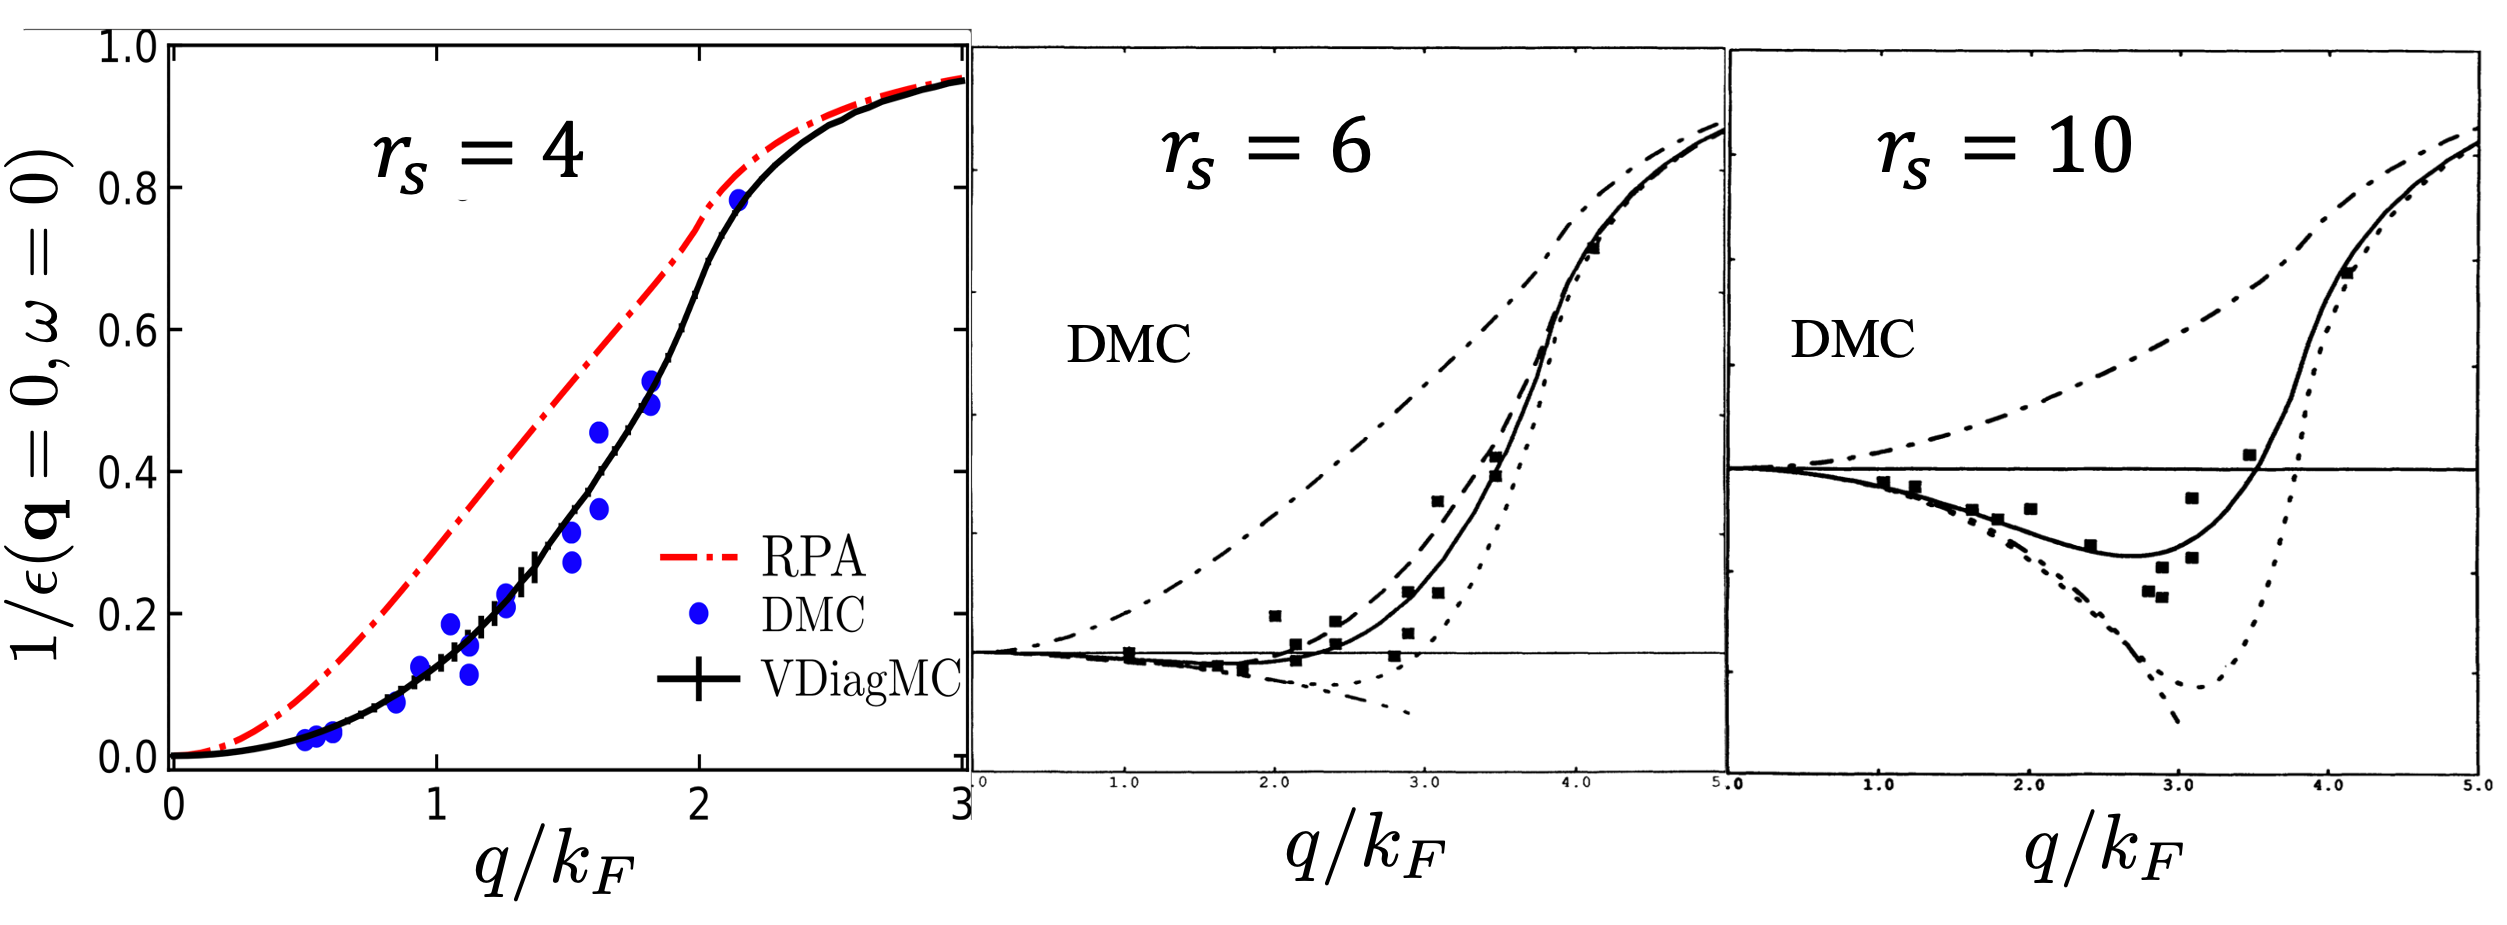
\includegraphics[width=\linewidth]{epsilon.png}
    \caption{The static dielectric function becomes negative near $r_s\approx 5.3$. The variational diagrammatic Monte Carlo (VDiagMC) data for $r_s=4$ is adapted from Ref.\citenum{kun}, while the diffusive quantum Monte Carlo (DMC) data for $r_s=4, 6, 10$ are adapted from Ref.\citenum{bowen}.}
\end{figure}

\begin{figure}
    \centering
    \resizebox{1.0\linewidth}{!}{
        \tikzset{every picture/.style={line width=0.75pt}} %set default line width to 0.75pt        

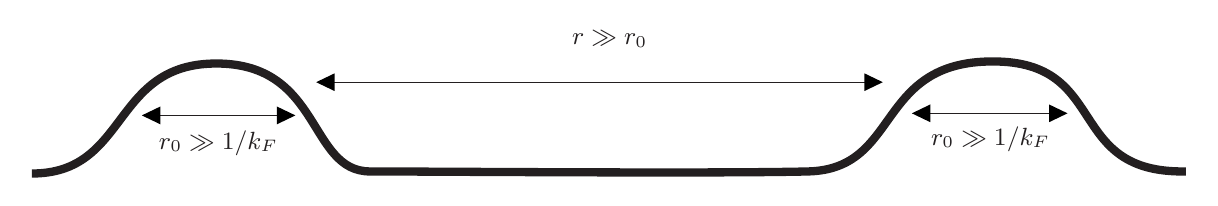
\begin{tikzpicture}[x=0.75pt,y=0.75pt,yscale=-1,xscale=1]
%uncomment if require: \path (0,300); %set diagram left start at 0, and has height of 300

%Curve Lines [id:da6730178697421663] 
\draw [line width=3]    (33,125) .. controls (80,125) and (71.06,71.93) .. (122,72) .. controls (172.94,72.07) and (166,124) .. (196,124) .. controls (226,124) and (361.98,125.09) .. (407,124) .. controls (452.02,122.91) and (439,71) .. (496,71) .. controls (553,71) and (530,125) .. (589,124) ;
%Straight Lines [id:da11185223986826509] 
\draw    (89,97) -- (157,97) ;
\draw [shift={(160,97)}, rotate = 180] [fill={rgb, 255:red, 0; green, 0; blue, 0 }  ][line width=0.08]  [draw opacity=0] (8.93,-4.29) -- (0,0) -- (8.93,4.29) -- cycle    ;
\draw [shift={(86,97)}, rotate = 0] [fill={rgb, 255:red, 0; green, 0; blue, 0 }  ][line width=0.08]  [draw opacity=0] (8.93,-4.29) -- (0,0) -- (8.93,4.29) -- cycle    ;
%Straight Lines [id:da08396554987934568] 
\draw    (460,96) -- (529,96) ;
\draw [shift={(532,96)}, rotate = 180] [fill={rgb, 255:red, 0; green, 0; blue, 0 }  ][line width=0.08]  [draw opacity=0] (8.93,-4.29) -- (0,0) -- (8.93,4.29) -- cycle    ;
\draw [shift={(457,96)}, rotate = 0] [fill={rgb, 255:red, 0; green, 0; blue, 0 }  ][line width=0.08]  [draw opacity=0] (8.93,-4.29) -- (0,0) -- (8.93,4.29) -- cycle    ;
%Straight Lines [id:da1160594665438861] 
\draw    (173,81) -- (440,81) ;
\draw [shift={(443,81)}, rotate = 180] [fill={rgb, 255:red, 0; green, 0; blue, 0 }  ][line width=0.08]  [draw opacity=0] (8.93,-4.29) -- (0,0) -- (8.93,4.29) -- cycle    ;
\draw [shift={(170,81)}, rotate = 0] [fill={rgb, 255:red, 0; green, 0; blue, 0 }  ][line width=0.08]  [draw opacity=0] (8.93,-4.29) -- (0,0) -- (8.93,4.29) -- cycle    ;

% Text Node
\draw (93,103) node [anchor=north west][inner sep=0.75pt]  [font=\small] [align=left] {$\displaystyle r_{0} \gg 1/k_{F}$};
% Text Node
\draw (292,55) node [anchor=north west][inner sep=0.75pt]  [font=\small] [align=left] {$\displaystyle r\gg r_{0}$};
% Text Node
\draw (465,101) node [anchor=north west][inner sep=0.75pt]  [font=\small] [align=left] {$\displaystyle r_{0} \gg 1/k_{F}$};


\end{tikzpicture}



    }
    \caption{Interaction between two clouds of test charge. The size of the cloud must be bigger than the inverse Fermi momentum. The separation of two clouds should be much larger than the size of the clouds.}
    \label{fig:test_charge}
\end{figure}


A particular interesting feature of the UEG is that the angle-averaged spin-symmetric Landau parameter $F_0^+$ approaches to $-1$ at $r_s \approx 5$, which corresponds to the density of akali metals. The system becomes bizarre in this limit. For example, the static dielectric function becomes negative in the limit $\bq \rightarrow 0$ when $F_0^+<-1$,
\begin{equation}
    \frac{1}{\epsilon_{\bq}} \xrightarrow{\bq \rightarrow 0} \frac{(1+F_0^+)\bq^2}{(q_{TF}^*)^2+(1+F_0^+)\bq^2}+O(\bq^4),
\end{equation}
where the $q_{TF}^*=\sqrt{4\pi e^2 N_F^*}$ with $N_F^*=\frac{m^*}{m}N_F$ the density of state of the quasiparticle on the Fermi surface.

Note that the negative dielectric function is compatible with the stability condition of the ground state\cite{dolgov},
\begin{equation}
    \frac{1}{\epsilon_{\bq}}<1,
\end{equation}
which means that the system could still be a stable Fermi liquid at $r_s\approx 5.3$.

Nevertheless, the negative dielectric causes physical consequences. As shown in Fig.\ref{fig:test_charge}, consider two clouds of test charges (say, two large impurities). The size of the clouds $r_0$ should be much larger than $1/k_F$ so that the short-wave-length effects such as the Fridel oscillation is suppressed. When the separation of the clouds are much larger than $r_0$, their static interaction is given by $v_\bq/\epsilon_\bq$ in the limit $\bq \ll k_F$, which is attractive for $r_s\lesssim 5.3$, and repulsive for $r_s \gtrsim 5.3$. Right at the density with $F_0^+=-1$, two test charge clouds are nearly free. In simple metals, the electrons provide the cohesive energy to bind the ions. The suppression of the test charge attraction is significant in akali metal, which may be strong enough to modify the lattice structure.

\subsection{Quasiparticle Interaction}

The nontrivial physics described in the above subsection originates from the collision process of two quasiparticles. The scattering amplitude is the probability that a given collision process happens. We will call the quasiparticle scattering amplitude as the quasiparticle interaction. Assume two quasiparitcles with momentum-frequency $k_1$ and $k_2$ are scatters to $k_3$ and $k_4=k_1+k_2-k_3$, the quasiparticle interaction is given by the one-particle irreducible (1PI) vertex function $z^2 \Gamma^4_{k_1, k_2; k_3, k_4}$ reweighted by the wave-function renormalization factor.

In a Fermi liquid, we expect that the quasiparticle interaction has a fast component and a slow component separated by the time scale $1/E_F$. The fast interaction comes from the bare Coulomb repulsion and high order quantum corrections under the length scales $1/k_F$. In addition to the fast process, two separated quasiparticles may also interact indirectly through the particle-hole excitations in the system, which generates a slow effective interaction.

The above consideration can be made exact for the forward scattering process. Indeed, one of the main predictions of Fermi liquid theory is that the forward scattering amplitudes on the Fermi surface are completely fixed the Fermi liquid parameters. In particular, the angle-averaged amplitude on the Fermi surface is given by,
\begin{equation}
    \label{eq:gamma_FL}
    z^2\overline{\Gamma^4_{k_1, k_2; k_1-q, k_2+q}}
    \xrightarrow[q \rightarrow 0]{}\frac{v_q+f_0^+}{1-(v_q+f_0^+)\Pi^*_0}+\frac{f_0^-}{1-f_0^-\Pi_0^*}\sigma\sigma',
\end{equation}
where the symbol $\overline{\Gamma_4}$ means projecting the incoming momentum-frequency to the Fermi surface $k_1=(0, k_F\mathbf{n}_1)$ and $k_2=(0, k_F\mathbf{n}_2)$, then average over the orientation of the unit vectors $\mathbf{n}_1$ and $\mathbf{n}_2$. The first term is the spin symmetric interaction, while the second term is spin asymmetric.

The norminators $v_q+f_0^+$ and $f_0^-$ in the scattering amplitude are the fast interaction. Except the Coulomb replusion, they are regular functions parameterized by the Landau parameter in the limit $q\rightarrow 0$: $f_0^\pm \rightarrow F_0^\pm N_F^*/z^2$. The fast interaction is then renormalized by a series of particle-hole pairs. The resummation of the particle-hole pairs generates the denorminators, where $\Pi_0^*(q)=\frac{m^*}{m}\Pi_0(q)$ with $\Pi_0(q)$ the momentum-frequency dependent Lindhard function. Note that $\Pi_0^*(q)$ is nonanalytic in the limit $q\rightarrow 0$ due to the charge conservation: $\Pi_0^*(q_0=0, \bq \rightarrow 0)=0$, while $\Pi_0^*(q_0\rightarrow 0, \bq = 0)=0$. As a result, the quasiparticle interaction in the forward scattering process has two distinct types of singularity: one is from the Coulomb repulsion, another is from the Lindhard function.

Landau Fermi liquid theory only specifies the forward scattering process. In Ref. \citenum{kukkonen}, Kukkonen and Overhauser propose to use a similar form as the Eq.\eqref{eq:gamma_FL} to parameterize the generic quasiparticle interactions,
\begin{equation}
    \label{eq:KO}
    R_q = \frac{v_q+f^+}{1-(v_q+f^+)\Pi^*_0}+\frac{f^-}{1-f^-\Pi_0^*}\sigma\sigma'+ u,
\end{equation}
where the counterterm $u$ should be included because some high-order quantum effects are doubly counted in the direct and the exchange interactions. The parameters $f^\pm$ and $u$ need to be carefully chosen to best approximate the physical scattering amplitude,
\begin{equation}
    z^2\Gamma^4_{k_1, k_2; k_1-q, k_2+q} \approx R_q - R_{q-k_1+k_2}
\end{equation}
up to the length scale $1/k_F$ and the time scale $1/E_F$.
%    -&\text{exchange interaction with $q \leftrightarrow q-k_1+k_2$}. 
The original Kukkonen-Overhauser (KO) formulation is a motivated by a phenomenological consideration based on the linear response theory. In literature, $f^\pm$ are parameterized as the exchange-correlation kernel $f_{xc}^\pm$ which can be extracted from the density-density and spin-spin response functions (See Fig. \ref{fig:fxc}) and the counterterm is set as $u=-f^+-f^-$. Note that such parameterization doesn't reproduce the Landau Fermi liquid theory Eq.\eqref{eq:gamma_FL} in the forward scattering process. The deviation could be significant near $r_s\approx 5.3$.

To fix this problem, we will use a parameterization where the spin-symmetric interaction in the forward scattering process is perfectly matches with the physical behavior:
\begin{equation}
    \label{eq:renorm_f1}
    f^+ \equiv F_0^\pm N_F^*/z^2,
\end{equation}
and the renormalization condition,
\begin{equation}
    \label{eq:renorm_f2}
    z^2\overline{\Gamma^{4}_{k_1, k_2; k_1-q, k_2+q}}^+ \equiv \overline{R_q}^+ - \overline{R_{q-k_1+k_2}}^+,
\end{equation}
where symbol $+$ means only the spin-symmetric part should be matched. As indicated by Fig. \ref{fig:fxc}, the quasiparticle interactions are local within the length scale $1/2k_F$, it then makes sense to choose $f^\pm$ and $u$ to be independent of the transfer momentum and frequency. Then the above renormalization conditions uniquely fixes all three parameters (See Appendix. \ref{appendix:renormalization} for more details).

\begin{figure}
    \centering
    \begin{subfigure}[b]{0.48\linewidth}
        \centering
        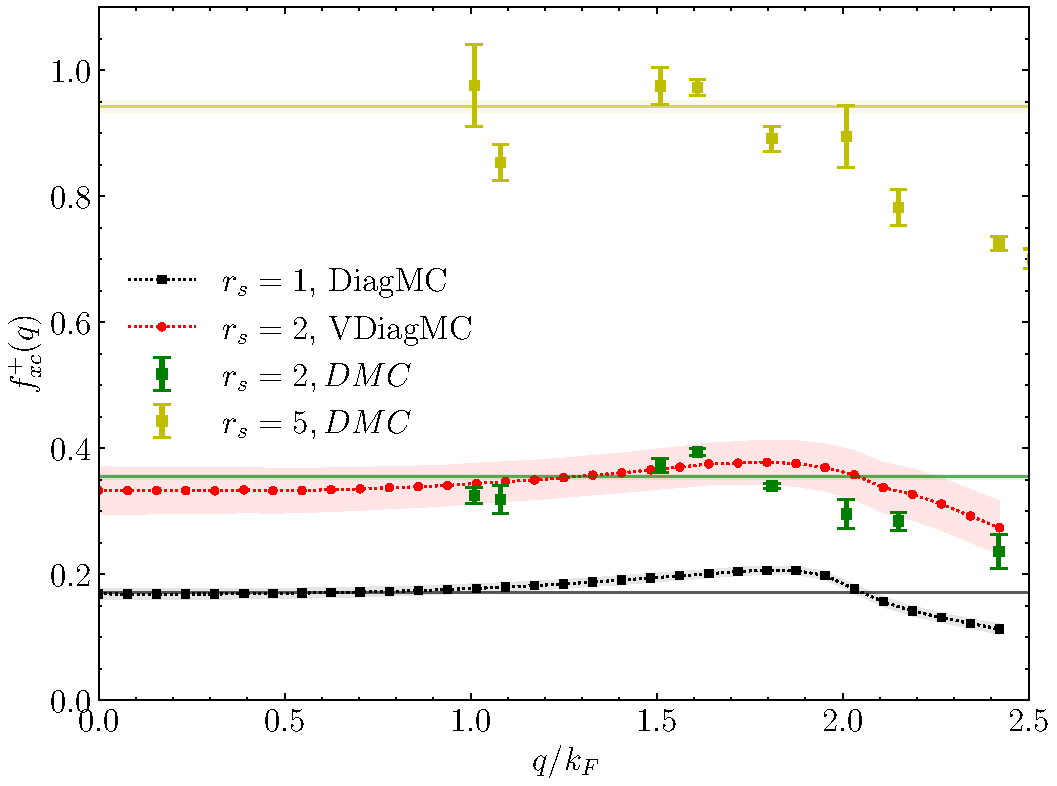
\includegraphics[width=\linewidth]{fxc_charge.pdf}
        %\caption{$charge$}
        \label{fig:charge_xc}
    \end{subfigure}
    %\hfill
    \begin{subfigure}[b]{0.48\linewidth}
        \centering
        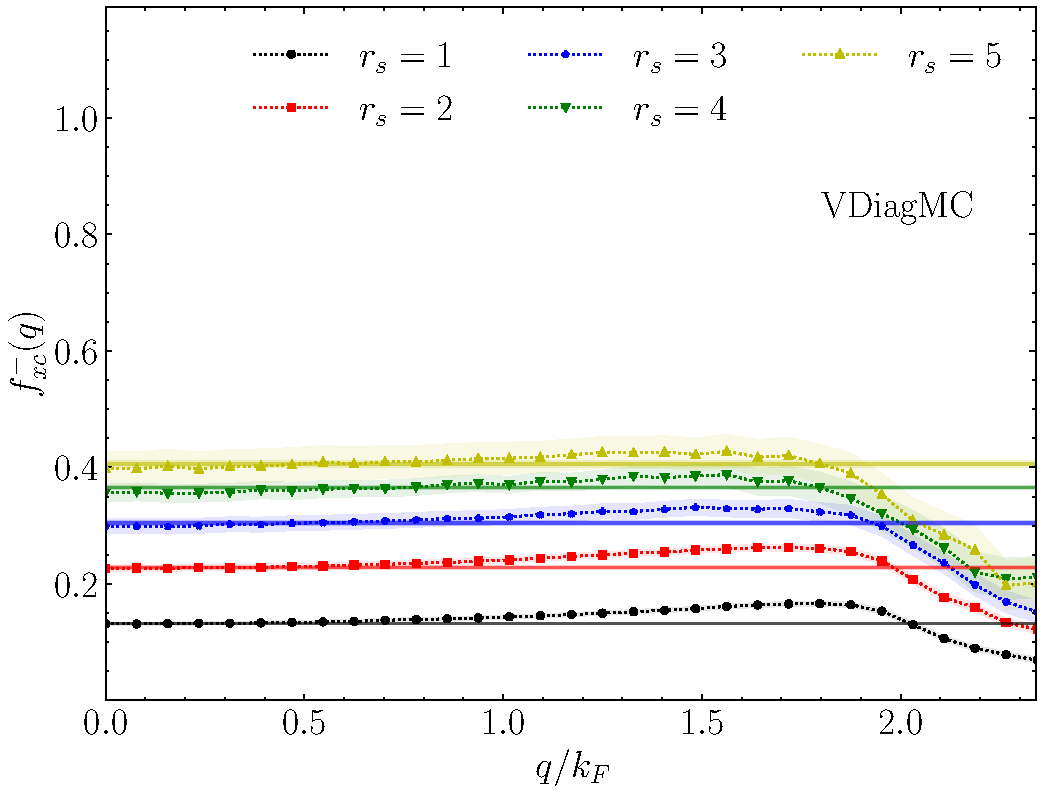
\includegraphics[width=\linewidth]{fxc_spin.pdf}
        %\caption{$spin$}
        \label{fig:spin_xc}
    \end{subfigure}
    \caption{Exchange-correlation kernel $f_{xc}^\pm$ as a function of the transfer momentum. Left: Spin-symmetric (charge) kernel calculated by diffusive quantum Monte Carlo (DMC) and variational diagrammatic Monte Carlo (VDiagMC). Right: Spin-asymmetric (spin) kernel calculated by VDiagMC. The vertical lines in both figures are the uniform exchange-correlation kernels extracted from the ground state energy obtained by DMC. Both $f_{xc}^\pm$ are relatively flat up the momentum $2k_F$, indicating that the exchange-correlation kernel is localized within the scale $1/2k_F$.}
    \label{fig:fxc}
\end{figure}

\section{Renormalized Field Theory}
\subsection{Effective Action}

In this subsection, we introduce a renormalized field theory based on the quasiparticle interaction ansatz proposed in the last subsection. It is the minimal theory that accounts for the essential vertex corrections for the physics near $r_s\approx 5.3$.

The attempt to describe Fermi liquid with a modern effective field theory approach was pioneered by Polchinski, Shankar and many other authors in Ref. \cite{polchinski1992effective, shankarRG, hewsonRG, dupuisRG,ChitovRG}). Here we further develop this idea. More specifically, we would like to write down a local EFT of a (charged Fermi liquid) which allows us to systematically derive physical observables. Some requirements are the following,

\begin{enumerate}
    \item The degrees of freedom of the EFT should be the quasiparticle instead of the bare electrons. The relation between our EFT and the jellium model (Eq.\eqref{eq:jellium}) is similar to that between the renormalized quantum electrodynamics (QED) and the bare theory defined above the Plank scale.

    \item The EFT should provide a unbiased description of the bare model in Eq.\eqref{eq:jellium}. That means we can not simply drop corrections as one usually did in condensed matter field theory. By systematically solving the EFT, one should be able to calculate the physical observable of the jellium model with a controlled estimation of errors. This is important because we want the theory to be useful as a first principle technique for real material calculations in the future.

    \item The EFT should keep all the symmetry (crossing symmetry, global $U(1)$ symmetry, Galilean symmetry, etc.) of the jellium model in Eq.\eqref{eq:jellium}. The global $U(1)$ symmetry implies the charge conservation law, which is implemented as the Ward–Takahashi identity in quantum correlators. Many of the renormalized perturbation theory violates such identity (for example, the polarization calculated from the fully self-consistent GW approximation). We want the perturbative treatment of our EFT to implement the Ward–Takahashi identity order by order.
\end{enumerate}

The minimal effective field theory that meets all three requirements are given by,
\begin{equation}
    \label{eq:renorm_action}
    S_R=\sum_{k \sigma} g_{R;k}^{-1}\bar{c}^R_{k \sigma} c^R_{k \sigma} + \frac{1}{2}\sum_{q\sigma, \bq \neq 0}  R_q \rho^R_{q\sigma} \rho^R_{-q\sigma},
\end{equation}
where $\bar{c}^R$ and $c^R$ are the Grassmann fields of quasiparticles. They are related to the bare electron fields $\bar{c}$ and $c$ in Eq. \eqref{eq:ueg_action} via a rescaling,
\begin{equation}
    \label{eq:rescaling}
    \bar{c}_{k\sigma} = \sqrt{z} \bar{c}^R_{k\sigma}, \quad c_{k\sigma} = \sqrt{z} c^R_{k\sigma},
\end{equation}
where $z$ is the wave-function renormalization factor.

The quasiparticle in the minimal theory has a renormalized propagator,
\begin{equation}
    \label{eq:gR}
    g_{R;k}=-\frac{1}{ik_0+\frac{\bk^2}{2m^*}-\mu_R},
\end{equation}
where the mass is renormalized to the effective mass $m^*$, and the chemical potential is chosen so that $g_R$ gives the electron density. Since we also rescale the quasiparticle fields with the factor $\sqrt{z}$, the quasiparticle spectral density has weight one.

Since the charge fluctuations dominate the physics for intermediate $r_s$, it is sufficient for us to only include the quasiparticle interaction only couples the density degrees of freedom,
\begin{equation}
    \label{eq:R}
    R_q=\frac{v_q+f^+}{1-(v_q+f^+)\Pi^*_0(q)}-f^+,
\end{equation}
where $\Pi_0^*(q)=\frac{m^*}{m}\Pi_0(q)$ with $\Pi_0(q)$ the momentum-frequency dependent Lindhard function. The parameters $f^+$ is the spin-symmetric Landau parameter. Such interaction reduces to the Landau Fermi liquid theory in the forward scattering channel up to a small regular correction. The tree level of our minimal theory already captures the nontrivial physics near $r_s=5.3$.

In principle, the system also develops effective spin-spin interaction between the quasiparticles. Our minimal model doesn't include the spin-spin quasiparticle interaction because they are rather small and can be treated perturbatively with high-order diagrams.

%As long as $f^+$ are nonzero, one can show that some of the vertex corrections have been double counted in the renormalized interaction $R_q$. An additional term must be present in the theory to compensate such double counting. Such term should be a contact interaction because the parameter $f^+$ in our minimal theory is independent of the transfer momentum and frequency. The only allowed possible term is then a Hubbard-like contact interaction $u$ in Eq.\ref{eq:renorm_action} between two quasiparticles with the opposite spins. 

\subsection{Renormalized Perturbation Theory}

In later sections, we will show how to use Feynman diagrammatic technique to systematically calculate the renormalized field theory. We will follow the standard procedure of renormalization technique in quantum field theory. A detailed introduction could be found the textbooks of quantum field theory, for example, Ref. \citenum{peskin1995quantum}.


\subsubsection{Counterterms}

We first connect the renormalized action to the bare action in Eq.\eqref{eq:ueg_action}. By rescaling the electron fields in the bare action to the quasiparticle fields using Eq.\eqref{eq:rescaling}, we obtain
\begin{equation}
    S_{UEG} = z\sum_{k \sigma} g_{k}^{-1}\bar{c}^R_{k \sigma} c^R_{k \sigma} + \frac{z^2}{2}\sum_{q\sigma, \bq \neq 0}  v_q \rho^R_{q\sigma} \rho^R_{-q\sigma}.
\end{equation}

The bare propagator and interaction still appear in the action, but they can be eliminated as follows,
\begin{equation}
    \label{eq:renorm_action}
    S_{UEG} = S_R + \sum_{k \sigma} \delta_g \bar{c}^R_{k \sigma} c^R_{k \sigma} + \frac{1}{2}\sum_{q\sigma, \bq \neq 0}  \delta_R \rho^R_{q\sigma} \rho^R_{-q\sigma}.
\end{equation}
The dominating term $S_R$ only involves the renormalized parameters. The remaining terms are known as the counterterms that have absorbed the shifts between the bare parameters and the physical parameters. One can show,
\begin{equation}
    \label{eq:ct1}
    \delta_g=z\cdot g_k^{-1}-g_{R; k}^{-1} \equiv -\delta_z ik_0-\delta_m \frac{\bk^2}{2m} +\delta_\mu,
\end{equation}
where,
\begin{equation}
    \label{eq:ct2}
    \delta_z=z-1, \quad \delta_m=z-\frac{m}{m^*},\quad  \delta_\mu=z\mu-\mu_R.
\end{equation}
In addition, the counterterm for the renormalized interaction is given by
\begin{equation}
    \label{eq:ct3}
    \delta_R = z^2 v_q - R_q.
\end{equation}

\subsubsection{Renormalization Conditions}

The definitions in Eq.\eqref{eq:ct2} and \eqref{eq:ct3} are not useful unless we give precise definitions of the renormalized parameters.

The renormalized parameters are defined through physical observables in terms of two-point and four-point vertex functions of the quasiparticle.
The two-point vertex function can be derived from the fully dressed propagator of the quasiparticle,
\begin{equation}
    G^R_k \equiv \left< \mathcal{T} \hat{c}_R(\tau_1 \mathbf{x}_1) \hat{c}_R^{\dag}(\tau_2 \mathbf{x}_2) \right>_k=\frac{1}{z}\left< \mathcal{T} \hat{c}(\tau_1 \mathbf{x}_1) \hat{c}^{\dag}(\tau_2 \mathbf{x}_2) \right>_k,
\end{equation}
so that the two-point vertex function of the quasiparticle,
\begin{equation}
    \Gamma^{2,R}_k = (G^R_k)^{-1}.
\end{equation}

According to the Landau Fermi liquid theory, $\Gamma^2_k$ should be analytic in the vicinity of the Fermi surface,
\begin{align*}
    \Gamma^{2,R}_k & \rightarrow -i k_0-\frac{\bold{k}_F}{m^*}\cdot(\bold{k}-\bold{k}_F)+O(\omega_n^2, (\bold{k}-\bold{k}_F)^2) \\
                   & \rightarrow -i k_0-\frac{\bold{k}^2}{2m^*}+E_F+O(\omega_n^2, (\bold{k}-\bold{k}_F)^2)
\end{align*}

The above equation leads to the following renormalization conditions that implicitly fixes the renormalized parameters $z$, $m^*$ and $\mu_R$.
For convenience, we introduce the quasiparticle self-energy
\begin{equation}
    \Sigma^{R}_k \equiv \Gamma^{2,R}_k-g_{R; k}
\end{equation}

\begin{enumerate}
    \item The renormalized chemical potential is fixed by,
          \begin{equation}
              \label{eq:condition1}
              \mu_R \equiv \operatorname{Re}\Gamma^{R;2}_{(0, k_F)} = E_F \rightarrow \operatorname{Re}\Sigma^{R}_{(0, k_F)} = 0
          \end{equation}

    \item The wave-function renormalization factor $z$ is implicitly fixed by the equation,
          \begin{equation}
              \label{eq:condition2}
              \frac{\partial }{\partial k_0}\left(\operatorname{Im} \Gamma^{R; 2}_{(0, k_F)}\right) = -1 \rightarrow \frac{\partial }{\partial k_0}\left(\operatorname{Im} \Sigma^{R}_{(0, k_F)}\right) = 0,
          \end{equation}
    \item The effective mass is fixed by both the small momentum and the frequency behavior of the self-energy near the Fermi surface,
          \begin{equation}
              \label{eq:condition3}
              \frac{m}{m^*}=-\frac{m}{k_F}\frac{\partial }{\partial \bold{k}}\left(\operatorname{Re}\Gamma^{R;2}_{(0, k_F)}\right) \rightarrow \frac{\partial }{\partial \bold{k}}\left(\operatorname{Re}\Sigma^{R}_{(0, k_F)}\right)=0.
          \end{equation}
\end{enumerate}

The remaining renormalized parameter $f^+$ is the Landau parameter of the quasiparticle interaction. It can be extracted from the two-quasiparticle scattering amplitude.
More specifically,  from the connected two-body Green's function of the quasiparticle,
\begin{equation}
    G^{c,R}_{k_1k_2; k_3k_4}\equiv \left< \mathcal{T} \hat{c}_R(\tau_1 \mathbf{x}_1)\hat{c}_R(\tau_2 \mathbf{x}_2) \hat{c}_R^\dag(\tau_3 \mathbf{x}_3)\hat{c}_R^\dag(\tau_4 \mathbf{x}_4) \right>^c_{k_1 k_2 k_3 k_3},
\end{equation}
one can derive the $4$-point 1PI vertex function, or the scattering amplitude, by amputating the two-body Green's function with the one-quasiparticle propagator,
\begin{equation}
    \Gamma^{4,R}_{k_1k_2;k_3k_4}\equiv G^{c,R}_{k_1k_2; k_3k_4}/\left[G^R_{k_1}G^R_{k_2}G^R_{k_3}G^R_{k_4}\right].
\end{equation}

The parameter $f^+$ is fixed to the spin-symmetric Landau parameter with $l=0$,
\begin{equation}
    \label{eq:condition4}
    f^+ = \left<\Gamma^{4,R}_{k_1, k_2; k_1-q, k_2+q}\right>_\Omega-v_q.
\end{equation}
where the symbol $\left<\Gamma_4\right>_\Omega$ is an operation with three steps:
i) project the incoming momentum-frequency to the Fermi surface $k_1=(0, k_F\mathbf{n}_1)$ and $k_2=(0, k_F\mathbf{n}_2)$,
ii) then send $q\rightarrow 0$ along the trajector $q_0 \gg v_F^*|\bq|$,
iii) and finally average over the orientation of the unit vectors $\mathbf{n}_1$ and $\mathbf{n}_2$.

The equations Eq. \eqref{eq:condition1},\eqref{eq:condition2}, \eqref{eq:condition3} and \eqref{eq:condition4} give the renormalization conditions to fix all renormalized parameters.


% where $\Gamma_4^\Omega$ is the quasiparticle scattering amplitude ($1PI$ vertex function) in the limit of zero transfer momentum $\mathbf{q}=0$ and small transfer frequency $\Omega \rightarrow 0$. The momenta and frequencies of two incoming electrons should be fixed on the Fermi surface. Note that the $l=0$ and spin-symmetric (denoted by the symbol $+$) component of $\Gamma_4^\Omega$ has a divergent term, which is bare Coulomb repulsion. This term must be subtracted to give the Landau parameter, which is regular. 


\subsubsection{Renormalized Perturbation Theory}

We will use a systematic perturbation technique to calculate the renormalized action Eq.\eqref{eq:renorm_action}. The procedure is known as renormalized perturbation theory.

The overall idea is to express a physical observable as a power series in the renormalized propagator and interaction. We may keep track of the perturbation order by associating the interaction with
\begin{equation}
    R_q \rightarrow R_q\xi,
\end{equation}
where $\xi$ should be set to be one in the end of the calculation.

To formulate a renormalized expansion, we first need to reparameterize the counterterms in Eq.\eqref{eq:ct2} and \eqref{eq:ct3} with the renormalized parameters.
They should be power series in the renormalized propagator $g_R$ and the interaction $R_q$. We first assume they can be expanded as,
\begin{equation}
    z=1+\sum_{n=1}^\infty z_n(g_R, R_q)\xi^n \leftrightarrow \delta_z= \sum_{n=1}^\infty z_n(g_R, R_q)\xi^n,
\end{equation}
where $z^{(n)}(g_R, R_g)$ is a multilinear functional of the renormalized propagator and the renormalized interaction with $n$ is the number of interaction lines. They are sum of renormalized Feynman diagrams.

Similarly,
\begin{equation}
    \frac{m}{m^*}=1+\sum_{n=1}^\infty m_n(g_R, R_q)\xi^n \leftrightarrow \delta_m= \sum_{n=1}^\infty \tilde{m}_n(g_R, R_q)\xi^n,
\end{equation}
where $\tilde{m}_n = z_n-m_n$.

Since we are not interested in the bare chemical potential of the system, we only need the power series for the chemical potential counterterm.
\begin{equation}
    \delta_\mu= \sum_{n=1}^\infty \mu_n(g_R, R_q)\xi^n
\end{equation}

Moreover, we need the power series of the Landau parameter,
\begin{equation}
    f^+= \sum_{n=1}^\infty f_n(g_R, R_q)\xi^n.
\end{equation}

To derive power series for the interaction counterterm $\delta_R$, one first needs to find the power series for the bare interaction $v_q$ in $R_q$.
According to the definition of the renormalized interaction Eq.\eqref{eq:R},
\begin{equation}
    v_q = \frac{R_q+f^+}{1+(R_q+f^+)\Pi_0^*}-f^+,
\end{equation}
Plugging it into Eq.\eqref{eq:ct3} and expanding in a power series in $R_q$, we obtain
\begin{align}
    \delta_R & =  z^2\left(\frac{R_q\xi+f^+}{1+(R_q\xi+f^+)\Pi_0^*}-f^+\right)\xi - R_q\xi \\
             & =           \left[2z_1 R_q-(R_q+f_1)^2\Pi_0^*\right]\xi^2+...
\end{align}
The physical meaning of terms will be clear later.

\subsubsection{Renormalized Feynman Diagrams}

\begin{figure}
    \centering
    \resizebox{0.8\linewidth}{!}{
        

\tikzset{every picture/.style={line width=0.75pt}} %set default line width to 0.75pt        

\begin{tikzpicture}[x=0.75pt,y=0.75pt,yscale=-1,xscale=1]
%uncomment if require: \path (0,532); %set diagram left start at 0, and has height of 532

%Straight Lines [id:da30552635388356797] 
\draw    (59,328) -- (107,261.5) ;
\draw [shift={(83,294.75)}, rotate = 125.82] [fill={rgb, 255:red, 0; green, 0; blue, 0 }  ][line width=0.08]  [draw opacity=0] (8.93,-4.29) -- (0,0) -- (8.93,4.29) -- cycle    ;
%Straight Lines [id:da29653976930952997] 
\draw    (107,261.5) -- (64,201.5) ;
\draw [shift={(85.5,231.5)}, rotate = 54.37] [fill={rgb, 255:red, 0; green, 0; blue, 0 }  ][line width=0.08]  [draw opacity=0] (8.93,-4.29) -- (0,0) -- (8.93,4.29) -- cycle    ;
%Shape: Wave [id:dp06516350314349983] 
\draw   (108,261.25) .. controls (109.79,265.48) and (111.51,269.5) .. (113.5,269.5) .. controls (115.49,269.5) and (117.21,265.48) .. (119,261.25) .. controls (120.79,257.02) and (122.51,253) .. (124.5,253) .. controls (126.49,253) and (128.21,257.02) .. (130,261.25) .. controls (131.79,265.48) and (133.51,269.5) .. (135.5,269.5) .. controls (137.49,269.5) and (139.21,265.48) .. (141,261.25) .. controls (142.79,257.02) and (144.51,253) .. (146.5,253) .. controls (148.49,253) and (150.21,257.02) .. (152,261.25) .. controls (153.79,265.48) and (155.51,269.5) .. (157.5,269.5) .. controls (159.49,269.5) and (161.21,265.48) .. (163,261.25) .. controls (164.79,257.02) and (166.51,253) .. (168.5,253) .. controls (170.49,253) and (172.21,257.02) .. (174,261.25) .. controls (175.79,265.48) and (177.51,269.5) .. (179.5,269.5) .. controls (181.49,269.5) and (183.21,265.48) .. (185,261.25) .. controls (186.79,257.02) and (188.51,253) .. (190.5,253) .. controls (192.49,253) and (194.21,257.02) .. (196,261.25) .. controls (197.79,265.48) and (199.51,269.5) .. (201.5,269.5) .. controls (203.49,269.5) and (205.21,265.48) .. (207,261.25) .. controls (208.79,257.02) and (210.51,253) .. (212.5,253) .. controls (214.49,253) and (216.21,257.02) .. (218,261.25) .. controls (219,263.62) and (219.98,265.92) .. (221,267.49) ;
%Straight Lines [id:da8891257908419108] 
\draw    (268,330) -- (220,263.5) ;
\draw [shift={(244,296.75)}, rotate = 54.18] [fill={rgb, 255:red, 0; green, 0; blue, 0 }  ][line width=0.08]  [draw opacity=0] (8.93,-4.29) -- (0,0) -- (8.93,4.29) -- cycle    ;
%Straight Lines [id:da9951539104533884] 
\draw    (220,263.5) -- (263,203.5) ;
\draw [shift={(241.5,233.5)}, rotate = 125.63] [fill={rgb, 255:red, 0; green, 0; blue, 0 }  ][line width=0.08]  [draw opacity=0] (8.93,-4.29) -- (0,0) -- (8.93,4.29) -- cycle    ;
%Straight Lines [id:da9467683455559888] 
\draw    (111,515) -- (159,448.5) ;
\draw [shift={(135,481.75)}, rotate = 125.82] [fill={rgb, 255:red, 0; green, 0; blue, 0 }  ][line width=0.08]  [draw opacity=0] (8.93,-4.29) -- (0,0) -- (8.93,4.29) -- cycle    ;
%Straight Lines [id:da13367315663371393] 
\draw    (159,448.5) -- (116,388.5) ;
\draw [shift={(137.5,418.5)}, rotate = 54.37] [fill={rgb, 255:red, 0; green, 0; blue, 0 }  ][line width=0.08]  [draw opacity=0] (8.93,-4.29) -- (0,0) -- (8.93,4.29) -- cycle    ;
%Straight Lines [id:da6726704779588752] 
\draw    (207,515) -- (159,448.5) ;
\draw [shift={(183,481.75)}, rotate = 54.18] [fill={rgb, 255:red, 0; green, 0; blue, 0 }  ][line width=0.08]  [draw opacity=0] (8.93,-4.29) -- (0,0) -- (8.93,4.29) -- cycle    ;
%Straight Lines [id:da5626412936723353] 
\draw    (159,448.5) -- (202,388.5) ;
\draw [shift={(180.5,418.5)}, rotate = 125.63] [fill={rgb, 255:red, 0; green, 0; blue, 0 }  ][line width=0.08]  [draw opacity=0] (8.93,-4.29) -- (0,0) -- (8.93,4.29) -- cycle    ;
%Shape: Circle [id:dp7660698888028996] 
\draw  [fill={rgb, 255:red, 0; green, 0; blue, 0 }  ,fill opacity=1 ] (151.5,448.5) .. controls (151.5,444.36) and (154.86,441) .. (159,441) .. controls (163.14,441) and (166.5,444.36) .. (166.5,448.5) .. controls (166.5,452.64) and (163.14,456) .. (159,456) .. controls (154.86,456) and (151.5,452.64) .. (151.5,448.5) -- cycle ;
%Straight Lines [id:da4225843171101724] 
\draw    (421,512) -- (469,445.5) ;
\draw [shift={(445,478.75)}, rotate = 125.82] [fill={rgb, 255:red, 0; green, 0; blue, 0 }  ][line width=0.08]  [draw opacity=0] (8.93,-4.29) -- (0,0) -- (8.93,4.29) -- cycle    ;
%Straight Lines [id:da2647368736134825] 
\draw    (469,445.5) -- (426,385.5) ;
\draw [shift={(447.5,415.5)}, rotate = 54.37] [fill={rgb, 255:red, 0; green, 0; blue, 0 }  ][line width=0.08]  [draw opacity=0] (8.93,-4.29) -- (0,0) -- (8.93,4.29) -- cycle    ;
%Straight Lines [id:da38769367934631704] 
\draw    (517,512) -- (469,445.5) ;
\draw [shift={(493,478.75)}, rotate = 54.18] [fill={rgb, 255:red, 0; green, 0; blue, 0 }  ][line width=0.08]  [draw opacity=0] (8.93,-4.29) -- (0,0) -- (8.93,4.29) -- cycle    ;
%Straight Lines [id:da46803848034211537] 
\draw    (469,445.5) -- (512,385.5) ;
\draw [shift={(490.5,415.5)}, rotate = 125.63] [fill={rgb, 255:red, 0; green, 0; blue, 0 }  ][line width=0.08]  [draw opacity=0] (8.93,-4.29) -- (0,0) -- (8.93,4.29) -- cycle    ;
%Shape: Circle [id:dp762976270046877] 
\draw   (461.5,445.5) .. controls (461.5,441.36) and (464.86,438) .. (469,438) .. controls (473.14,438) and (476.5,441.36) .. (476.5,445.5) .. controls (476.5,449.64) and (473.14,453) .. (469,453) .. controls (464.86,453) and (461.5,449.64) .. (461.5,445.5) -- cycle ;
%Straight Lines [id:da6551096511735701] 
\draw    (363,324) -- (411,257.5) ;
\draw [shift={(387,290.75)}, rotate = 125.82] [fill={rgb, 255:red, 0; green, 0; blue, 0 }  ][line width=0.08]  [draw opacity=0] (8.93,-4.29) -- (0,0) -- (8.93,4.29) -- cycle    ;
%Straight Lines [id:da10990492116983264] 
\draw    (411,257.5) -- (368,197.5) ;
\draw [shift={(389.5,227.5)}, rotate = 54.37] [fill={rgb, 255:red, 0; green, 0; blue, 0 }  ][line width=0.08]  [draw opacity=0] (8.93,-4.29) -- (0,0) -- (8.93,4.29) -- cycle    ;
%Shape: Wave [id:dp4341152704829403] 
\draw   (412,257.25) .. controls (413.79,261.48) and (415.51,265.5) .. (417.5,265.5) .. controls (419.49,265.5) and (421.21,261.48) .. (423,257.25) .. controls (424.79,253.02) and (426.51,249) .. (428.5,249) .. controls (430.49,249) and (432.21,253.02) .. (434,257.25) .. controls (435.79,261.48) and (437.51,265.5) .. (439.5,265.5) .. controls (441.49,265.5) and (443.21,261.48) .. (445,257.25) .. controls (446.79,253.02) and (448.51,249) .. (450.5,249) .. controls (452.49,249) and (454.21,253.02) .. (456,257.25) .. controls (457.79,261.48) and (459.51,265.5) .. (461.5,265.5) .. controls (463.49,265.5) and (465.21,261.48) .. (467,257.25) .. controls (468.79,253.02) and (470.51,249) .. (472.5,249) .. controls (474.49,249) and (476.21,253.02) .. (478,257.25) .. controls (479.79,261.48) and (481.51,265.5) .. (483.5,265.5) .. controls (485.49,265.5) and (487.21,261.48) .. (489,257.25) .. controls (490.79,253.02) and (492.51,249) .. (494.5,249) .. controls (496.49,249) and (498.21,253.02) .. (500,257.25) .. controls (501.79,261.48) and (503.51,265.5) .. (505.5,265.5) .. controls (507.49,265.5) and (509.21,261.48) .. (511,257.25) .. controls (512.79,253.02) and (514.51,249) .. (516.5,249) .. controls (518.49,249) and (520.21,253.02) .. (522,257.25) .. controls (523,259.62) and (523.98,261.92) .. (525,263.49) ;
%Straight Lines [id:da9012908623026843] 
\draw    (572,326) -- (524,259.5) ;
\draw [shift={(548,292.75)}, rotate = 54.18] [fill={rgb, 255:red, 0; green, 0; blue, 0 }  ][line width=0.08]  [draw opacity=0] (8.93,-4.29) -- (0,0) -- (8.93,4.29) -- cycle    ;
%Straight Lines [id:da8377345642414153] 
\draw    (524,259.5) -- (567,199.5) ;
\draw [shift={(545.5,229.5)}, rotate = 125.63] [fill={rgb, 255:red, 0; green, 0; blue, 0 }  ][line width=0.08]  [draw opacity=0] (8.93,-4.29) -- (0,0) -- (8.93,4.29) -- cycle    ;
%Shape: Circle [id:dp18254269642930243] 
\draw  [fill={rgb, 255:red, 255; green, 255; blue, 255 }  ,fill opacity=1 ] (458,259) .. controls (458,252.37) and (463.37,247) .. (470,247) .. controls (476.63,247) and (482,252.37) .. (482,259) .. controls (482,265.63) and (476.63,271) .. (470,271) .. controls (463.37,271) and (458,265.63) .. (458,259) -- cycle ;
%Straight Lines [id:da28378668601652346] 
\draw    (463,250) -- (478,268) ;
%Straight Lines [id:da18890855693648545] 
\draw    (463,267.25) -- (477,250.75) ;
%Straight Lines [id:da6156970647937039] 
\draw    (70,109) -- (269,108) ;
\draw [shift={(169.5,108.5)}, rotate = 179.71] [fill={rgb, 255:red, 0; green, 0; blue, 0 }  ][line width=0.08]  [draw opacity=0] (8.93,-4.29) -- (0,0) -- (8.93,4.29) -- cycle    ;
%Straight Lines [id:da5960709649805054] 
\draw    (358,107) -- (557,106) ;
\draw [shift={(457.5,106.5)}, rotate = 179.71] [fill={rgb, 255:red, 0; green, 0; blue, 0 }  ][line width=0.08]  [draw opacity=0] (8.93,-4.29) -- (0,0) -- (8.93,4.29) -- cycle    ;
%Shape: Circle [id:dp8730422063342325] 
\draw  [fill={rgb, 255:red, 255; green, 255; blue, 255 }  ,fill opacity=1 ] (461,107) .. controls (461,100.37) and (466.37,95) .. (473,95) .. controls (479.63,95) and (485,100.37) .. (485,107) .. controls (485,113.63) and (479.63,119) .. (473,119) .. controls (466.37,119) and (461,113.63) .. (461,107) -- cycle ;
%Straight Lines [id:da913926660260955] 
\draw    (466,98) -- (481,116) ;
%Straight Lines [id:da48816970476766186] 
\draw    (466,115.25) -- (480,98.75) ;


% Text Node
\draw (134,197.4) node [anchor=north west][inner sep=0.75pt]  [font=\LARGE]  {$\frac{1}{z^{2}} R_{q}^{\alpha }$};
% Text Node
\draw (68,248.4) node [anchor=north west][inner sep=0.75pt]  [font=\LARGE]  {$\sigma ^{\alpha }$};
% Text Node
\draw (236,245.4) node [anchor=north west][inner sep=0.75pt]  [font=\LARGE]  {$\sigma ^{\alpha }$};
% Text Node
\draw (147,379.4) node [anchor=north west][inner sep=0.75pt]  [font=\LARGE]  {$\frac{u}{z^{2}}$};
% Text Node
\draw (458,376.4) node [anchor=north west][inner sep=0.75pt]  [font=\LARGE]  {$\delta _{u}$};
% Text Node
\draw (459,206.4) node [anchor=north west][inner sep=0.75pt]  [font=\LARGE]  {$\delta _{R}$};
% Text Node
\draw (372,244.4) node [anchor=north west][inner sep=0.75pt]  [font=\LARGE]  {$\sigma ^{\alpha }$};
% Text Node
\draw (540,240.4) node [anchor=north west][inner sep=0.75pt]  [font=\LARGE]  {$\sigma ^{\alpha }$};
% Text Node
\draw (151,60.4) node [anchor=north west][inner sep=0.75pt]  [font=\LARGE]  {$g_{R}$};
% Text Node
\draw (463,54.4) node [anchor=north west][inner sep=0.75pt]  [font=\LARGE]  {$\delta _{g}$};


\end{tikzpicture}


    }
    \caption{Feynman rules for the renormalized field theory of the electron gas.}
    \label{fig:component}
\end{figure}

\begin{figure}
    \centering
    \begin{subfigure}{\linewidth}
        \resizebox{0.9\linewidth}{!}{
            \begin{axopicture}(684,189) (166,-265)
  \SetWidth{2.0}
  \SetColor{Black}
  \Line[arrow,arrowpos=0.5,arrowlength=10,arrowwidth=5,arrowinset=0.2](207,-259)(256,-164)
  \Line[arrow,arrowpos=0.5,arrowlength=10,arrowwidth=5,arrowinset=0.2](256,-164)(209,-84)
  \Line[arrow,arrowpos=0.5,arrowlength=10,arrowwidth=5,arrowinset=0.2](416,-263)(368,-163)
  \Line[arrow,arrowpos=0.5,arrowlength=10,arrowwidth=5,arrowinset=0.2](367,-162)(417,-82)
  \Photon(256,-164)(368,-162){7.5}{6}
  \Text(289,-207)[lb]{\Huge{\Black{$R_q$}}}
  \Text(183,-257)[lb]{\Huge{\Black{$k_1$}}}
  \Text(419,-257)[lb]{\Huge{\Black{$k_2$}}}
  \Text(140,-103)[lb]{\Huge{\Black{$k_1-q$}}}
  \Text(421,-100)[lb]{\Huge{\Black{$k_2+q$}}}
  \Line[arrow,arrowpos=0.5,arrowlength=10,arrowwidth=5,arrowinset=0.2](601,-260)(650,-165)
  \Line[arrow,arrowpos=0.5,arrowlength=10,arrowwidth=5,arrowinset=0.2](650,-165)(810,-77)
  \Line[arrow,arrowpos=0.5,arrowlength=10,arrowwidth=5,arrowinset=0.2](810,-264)(762,-164)
  \Line[arrow,arrowpos=0.5,arrowlength=10,arrowwidth=5,arrowinset=0.2](761,-163)(607,-77)
  \Text(575,-257)[lb]{\Huge{\Black{$k_1$}}}
  \Text(813,-257)[lb]{\Huge{\Black{$k_2$}}}
  \Text(555,-104)[lb]{\Huge{\Black{$k_1-q$}}}
  \Text(815,-101)[lb]{\Huge{\Black{$k_2+q$}}}
  \Photon(650,-165)(762,-163){7.5}{6}
  \Text(640,-207)[lb]{\Huge{\Black{$-R_{-q+k_2-k_1}$}}}
  \Text(500,-163)[lb]{\Huge{\Black{$+$}}}
\end{axopicture}
        }
        \caption{ }
    \end{subfigure}
    \begin{subfigure}{\linewidth}
        \resizebox{0.75\linewidth}{!}{
            \begin{axopicture}(537,132) (120,-103)
    \SetWidth{2.0}
    \SetColor{Black}
    \Line[arrow,arrowpos=0.5,arrowlength=10,arrowwidth=8,arrowinset=0.2](128,-92)(368,-92)
    \PhotonArc[clock](248,-100)(120.266,176.186,3.814){7.5}{18.5}
    \Line[arrow,arrowpos=0.5,arrowlength=5,arrowwidth=2,arrowinset=0.2](480,-88)(656,-88)
    \COval(570,-88)(14.142,14.142)(45.0){Black}{White}\Line(562.929,-95.071)(577.071,-80.929)\Line(562.929,-80.929)(577.071,-95.071)
    \Text(240,-48)[lb]{\Huge{\Black{$\Sigma_1$}}}
    \Text(560,-48)[lb]{\Huge{\Black{$\delta_g^1$}}}
    \Text(420,-70)[lb]{\Huge{\Black{$+$}}}
\end{axopicture}


        }
        \caption{ }
    \end{subfigure}
    \caption{The first order renormalized diagrams and their counterterms.
        a) Quasiparticle $4$-point vertex function.
        b) Quasiparticle self-energy. The Hatree diagram is neglected since it merely shifts the chemical potential.}
    \label{fig:order1}
\end{figure}

\begin{figure}
    \centering
    \begin{subfigure}{\linewidth}
        \resizebox{0.75\linewidth}{!}{
            \begin{axopicture}(543,847) (303,-235)
  \SetWidth{2.0}
  \SetColor{Black}
  \Text(592,522)[lb]{\Huge{\Black{$+$}}}
  \Text(385,515)[lb]{\Huge{\Black{$\gamma_2^{1d}$}}}
  \SetWidth{2.0}
  \Line[arrow,arrowpos=0.5,arrowlength=10,arrowwidth=5,arrowinset=0.2](669,461)(700,527)
  \Line[arrow,arrowpos=0.5,arrowlength=10,arrowwidth=5,arrowinset=0.2](700,527)(669,590)
  \Line[arrow,arrowpos=0.5,arrowlength=10,arrowwidth=5,arrowinset=0.2](843,463)(813,529)
  \Line[arrow,arrowpos=0.5,arrowlength=10,arrowwidth=5,arrowinset=0.2](814,529)(845,592)
  \Text(695,565)[lb]{\huge{\Black{$(z_1-f_1\Pi_0^*) R_q$}}}
  \Photon(697,527)(812,528){7.5}{6}
  \COval(755,527)(11.314,11.314)(45.0){Black}{White}\Line(749.343,521.343)(760.657,532.657)\Line(749.343,532.657)(760.657,521.343)
  \Line[arrow,arrowpos=0.5,arrowlength=10,arrowwidth=5,arrowinset=0.2](664,230)(695,296)
  \Line[arrow,arrowpos=0.5,arrowlength=10,arrowwidth=5,arrowinset=0.2](695,296)(664,359)
  \Line[arrow,arrowpos=0.5,arrowlength=10,arrowwidth=5,arrowinset=0.2](838,232)(808,298)
  \Line[arrow,arrowpos=0.5,arrowlength=10,arrowwidth=5,arrowinset=0.2](809,298)(840,361)
  \Text(697,329)[lb]{\huge{\Black{$R_q(z_1-f_1\Pi_0^*)$}}}
  \Photon(696,296)(807,297){7.5}{6}
  \COval(750,296)(11.314,11.314)(45.0){Black}{White}\Line(744.343,290.343)(755.657,301.657)\Line(744.343,301.657)(755.657,290.343)
  \Line[arrow,arrowpos=0.5,arrowlength=10,arrowwidth=5,arrowinset=0.2](309,231)(340,300)
  \Line[arrow,arrowpos=0.5,arrowlength=10,arrowwidth=5,arrowinset=0.2](340,302)(307,374)
  \Line[arrow,arrowpos=0.5,arrowlength=10,arrowwidth=5,arrowinset=0.2](546,230)(513,279)
  \Line[arrow,arrowpos=0.5,arrowlength=10,arrowwidth=5,arrowinset=0.2](512,335)(546,373)
  \Photon(341,300)(387,300){7.5}{2}
  \Arc[arrow,arrowpos=0.5,arrowlength=10,arrowwidth=5,arrowinset=0.2](461.85,274.102)(78.009,49.027,159.045)
  \Arc[arrow,arrowpos=0.5,arrowlength=10,arrowwidth=5,arrowinset=0.2](460.962,338.063)(80.129,-150.823,-48.554)
  \Photon(512,334)(516,278){5}{3}
  \Text(445,289)[lb]{\Huge{\Black{$\gamma_2^{2d}$}}}
  \Text(592,286)[lb]{\Huge{\Black{$+$}}}
  \Text(592,85)[lb]{\Huge{\Black{$+$}}}
  \Line[arrow,arrowpos=0.5,arrowlength=10,arrowwidth=5,arrowinset=0.2](305,26)(340,76)
  \Line[arrow,arrowpos=0.5,arrowlength=10,arrowwidth=5,arrowinset=0.2](337,127)(304,171)
  \Line[arrow,arrowpos=0.5,arrowlength=10,arrowwidth=5,arrowinset=0.2](544,32)(530,71)
  \Line[arrow,arrowpos=0.5,arrowlength=10,arrowwidth=5,arrowinset=0.2](528,126)(548,161)
  \Arc[arrow,arrowpos=0.5,arrowlength=10,arrowwidth=5,arrowinset=0.2](413.836,33.919)(122.246,18.15,128.942)
  \Arc[arrow,arrowpos=0.5,arrowlength=10,arrowwidth=5,arrowinset=0.2](411.245,184.969)(130.801,-121.964,-26.797)
  \Photon(339,126)(339,75){5}{3}
  \Photon(484,130)(487,77){4.5}{3}
  \Line[arrow,arrowpos=0.5,arrowlength=10,arrowwidth=5,arrowinset=0.2](318,453)(343,496)
  \Line[arrow,arrowpos=0.5,arrowlength=10,arrowwidth=5,arrowinset=0.2](343,551)(316,589)
  \Line[arrow,arrowpos=0.5,arrowlength=10,arrowwidth=5,arrowinset=0.2](547,459)(513,526)
  \Line[arrow,arrowpos=0.5,arrowlength=10,arrowwidth=5,arrowinset=0.2](513,526)(547,589)
  \Arc[arrow,arrowpos=0.5,arrowlength=10,arrowwidth=5,arrowinset=0.2](393.594,556.763)(79.21,-128.764,-22.07)
  \Arc[arrow,arrowpos=0.5,arrowlength=10,arrowwidth=5,arrowinset=0.2](396.293,492.371)(79.176,26.743,133.293)
  \Photon(467,527)(513,527){7.5}{2}
  \Photon(343,552)(345,497){5}{3}
  \Text(410,95)[lb]{\Huge{\Black{$\gamma_2^{3d}$}}}
  \Line[arrow,arrowpos=0.5,arrowlength=10,arrowwidth=5,arrowinset=0.2](663,30)(694,96)
  \Line[arrow,arrowpos=0.5,arrowlength=10,arrowwidth=5,arrowinset=0.2](694,96)(663,159)
  \Line[arrow,arrowpos=0.5,arrowlength=10,arrowwidth=5,arrowinset=0.2](837,32)(807,98)
  \Line[arrow,arrowpos=0.5,arrowlength=10,arrowwidth=5,arrowinset=0.2](808,98)(839,161)
  \Text(720,134)[lb]{\huge{\Black{$-f_1\Pi_0^*f_1$}}}
  \Photon(695,96)(806,97){7.5}{6}
  \COval(749,96)(11.314,11.314)(45.0){Black}{White}\Line(743.343,90.343)(754.657,101.657)\Line(743.343,101.657)(754.657,90.343)
  \Text(408,-140)[lb]{\Huge{\Black{$\gamma_2^{4d}$}}}
  \Line[arrow,arrowpos=0.5,arrowlength=10,arrowwidth=5,arrowinset=0.2](375,-234)(392,-192)
  \Line[arrow,arrowpos=0.5,arrowlength=10,arrowwidth=5,arrowinset=0.2](471,-233)(456,-189)
  \Arc[arrow,arrowpos=0.5,arrowlength=10,arrowwidth=5,arrowinset=0.2,clock](441.565,-131.828)(78.891,-127.995,-228.219)
  \Arc[arrow,arrowpos=0.5,arrowlength=10,arrowwidth=5,arrowinset=0.2](408.546,-130.6)(76.812,-51.844,50.889)
  \Line[arrow,arrowpos=0.5,arrowlength=10,arrowwidth=5,arrowinset=0.2](458,-70)(476,-37)
  \Line[arrow,arrowpos=0.5,arrowlength=10,arrowwidth=5,arrowinset=0.2](389,-73)(372,-35)
  \Photon(389,-73)(458,-70){5}{4}
  \Photon(392,-192)(458,-189){5}{4}
\end{axopicture}


        }
        \caption{}
    \end{subfigure}
    \begin{subfigure}{\linewidth}
        \resizebox{0.75\linewidth}{!}{
            %%%%%%%%%%%%%%%%%%%%%%%%%%%%%%%%%%%%%%%%%%%%%%%%%%%%%%%%%%%%%%%%%%%%%%%%%%%
%%%		LaTex file generated by JaxoDraw-2.1-0
%%%			CreationDate: 8/4/2022
%%%	Make sure you have the axodraw4j package installed in order to proceed!
%%%%%%%%%%%%%%%%%%%%%%%%%%%%%%%%%%%%%%%%%%%%%%%%%%%%%%%%%%%%%%%%%%%%%%%%%%%

% \documentclass[a4paper]{article}

% \usepackage{color}
% \usepackage{axodraw4j}
% \usepackage{pstricks}

% \setlength{\oddsidemargin}{0pt}
% \setlength{\evensidemargin}{0pt}
% \setlength{\topmargin}{0pt}
% \setlength{\headheight}{0pt}
% \setlength{\headsep}{0pt}
% \setlength{\topskip}{0pt}
% \setlength{\footskip}{0pt}
% \setlength{\textwidth}{\paperwidth}
% \addtolength{\textwidth}{-2in}
% \setlength{\textheight}{\paperheight}
% \addtolength{\textheight}{-2in}

% \pagestyle{empty}



% \begin{document}

% %%JaxoComment:
% %%JaxoScale{1.0}


% \begin{center}
% \fcolorbox{white}{white}{
\begin{axopicture}(590,530) (169,-137)
  \SetWidth{2.0}
  \SetColor{Black}
  \Line[arrow,arrowpos=0.5,arrowlength=12.5,arrowwidth=5,arrowinset=0.2](176,274)(416,274)
  \PhotonArc[clock](296,265.714)(120.286,176.05,3.95){6}{18.5}
  \PhotonArc[clock](296,266.5)(56.5,172.372,7.628){6}{8.5}
  \Text(272,344)[lb]{\Huge{\Black{$\Sigma_2^1$}}}
  \Line[arrow,arrowpos=0.5,arrowlength=12.5,arrowwidth=5,arrowinset=0.2](176,82)(416,82)
  \PhotonArc[clock](271.5,63.8)(98.201,169.319,10.681){6}{14.5}
  \PhotonArc(328,90.4)(88.4,-174.547,-5.453){6}{13.5}
  \Text(272,104)[lb]{\Huge{\Black{$\Sigma_2^3$}}}
  \Line[arrow,arrowpos=0.5,arrowlength=12.5,arrowwidth=5,arrowinset=0.2](512,82)(752,82)
  \Text(656,200)[lb]{\Huge{\Black{$\delta_R^2$}}}
  \PhotonArc[clock](632,73.714)(120.286,176.05,3.95){6}{18.5}
  \Text(608,334)[lb]{\Huge{\Black{$\Sigma_2^2$}}}
  \Line[arrow,arrowpos=0.5,arrowlength=12.5,arrowwidth=5,arrowinset=0.2](512,274)(752,274)
  \COval(640,274)(14.142,14.142)(45.0){Black}{White}\Line(632.929,266.929)(647.071,281.071)\Line(632.929,281.071)(647.071,266.929)
  \Text(596,236)[lb]{\Huge{\Black{$\delta_g^1$}}}
  \PhotonArc[clock](632,265.714)(120.286,176.05,3.95){6}{18.5}
  \COval(640,194)(14.142,14.142)(45.0){Black}{White}\Line(632.929,186.929)(647.071,201.071)\Line(632.929,201.071)(647.071,186.929)
  \Text(608,104)[lb]{\Huge{\Black{$\Sigma_2^4$}}}
  \Line[arrow,arrowpos=0.5,arrowlength=12.5,arrowwidth=5,arrowinset=0.2](373,-121)(533,-121)
  \COval(453,-121)(14.142,14.142)(45.0){Black}{White}\Line(445.929,-128.071)(460.071,-113.929)\Line(445.929,-113.929)(460.071,-128.071)
  \Text(437,-89)[lb]{\Huge{\Black{$\delta_g^2$}}}
\end{axopicture}
% }
% \end{center}

% \end{document}


        }
        \caption{ }
    \end{subfigure}
    \caption{The second order renormalized diagrams and their counterterms.
        a) Quasiparticle $4$-point vertex function. Each diagram and counterterm has an
        exchange counterpart by swapping the two outgoing quasiparticles. The bubble diagram is completely
        canceled out by the counterterm, thus not included.
        b) Quasiparticle self-energy.}
    \label{fig:order2}
\end{figure}


Now we have all components to formulate the renormalized perturbation theory in terms of renormalized Feynman diagrams.
The building blocks of the diagrams are given in Fig.\eqref{fig:component}. By organizing the
diagrams in number of renormalized interactions (namely, in order of $\xi$),
we derive the first two orders of renormalized Feynman diagrams for the quasiparticle
self-energy and scattering amplitudein in Fig.\ref{fig:order1} and Fig.\ref{fig:order2}.

We first discuss the first order diagrams in Fig.\ref{fig:order1}. They give the leading order
estimation of the renormalized parameters. Fig.\ref{fig:order1}(a) is for the $4$-point vertex function
$\Gamma^{4,R}_{k_1, k_2; k_1-q, k_2+q}$. Averaging it on the Fermi surface using Eq.\eqref{eq:condition4}
gives the leading order of the Landau parameter,
\begin{equation}
    f_1 = -\left< R_{-q+k_2-k_1}\right>_\Omega.
\end{equation}
Note that the direct interaction doesn't contribute to $f_1$ because
$\left<R_q\right>=v_q$ and the bare Coulomb interation is not part of the Landau parameter.

The leading order quasiparticle self-energy is shown in Fig.\eqref{fig:order1}(b).
It is the first example of diagrams that comes with a counterterm $\delta_g^1$. The sum of the diagram
and the counterterm should satisfy the renormalization condition Eq.\eqref{eq:condition1}, \eqref{eq:condition2} and \eqref{eq:condition3}.
We conclude the leading order correction to the $z$-factor is
\begin{equation}
    z_1 = \left. \frac{\partial \operatorname{Im} \Sigma_1}{\partial k_0} \right|_{(0, k_F)},
\end{equation}
where $\Sigma_1$ is the Fock diagram (the left diagram in Fig.\eqref{fig:order1}(b)).

Similarly, the effective mass counterterm should be
\begin{equation}
    \tilde{m}_1 = \frac{m}{k_F}\left. \frac{\partial \operatorname{Re} \Sigma_1}{\partial \bold{k}} \right|_{(0, k_F)}.
\end{equation}
The leading order correction to the effective mass is
\begin{equation}
    m_1 = z_1+\tilde{m}_1.
\end{equation}
In addition, the chemical potential counterterm should remove the chemical-potential shift from the self-energy diagram, therefore,
\begin{equation}
    \delta \mu_1 = -\operatorname{Re} \Sigma_1(0, k_F).
\end{equation}

The above procedure can be systematically performed for the second order corrections.
As shown in Fig.\ref{fig:order2}, the second order Feynman diagrams come with sophisticated counterterms.
For the $4$-point vertex function diagrams, the interaction counterterm $\delta_R^2$ appears for the first time.
For clarity, we split $\delta_R^2$ into three parts, each of which is paired with a renormalized Feynman diagram.
For example, the diagram $\gamma_2^{1d}$, which is a left vertex correction diagram, is paired with the counterterm $z_1R_q-f1\Pi^*_0R_q$.
The physical meaning is clear: $z_1 R_q$ canecels out the regular contribution in the left vertex correction,
while $f_1\Pi_0^*R_q$ cancels out the non-analytic contribution from a particle-hole pair.

Using the renormalization condition in Eq.\eqref{eq:condition4}, we derive the second-order correction to the Landau parameter,
\begin{equation}
    f_2 = \left<\gamma_2^{3d}+\gamma_2^{4d}+\gamma_2^{1e}+\gamma_2^{2e}+\gamma_2^{3e}+\gamma_2^{4e} + \text{CT}\right>_\Omega.
\end{equation}
Note that only the proper diagrams (one-interaction-irreducible) diagrams contribute to $f^+$.

The second-order self-energy diagrams and their counterterms are shown in Fig.\ref{fig:order2}(b).
They fix the corrections $z_2$, $m_2$ and $\mu_2$. We will not repeat the analysis here.

\section{Charge Instability in the Charged Fermi liquid Theory}

Here we review the two-particle properties of the charged Fermi liquid in the context of the electron gas problem Eq.\eqref{eq:jellium}. We are particularly interested in the potential instability in the particle-hole channel.

In a Fermi liquid, the low-energy dynamics of the quasiparticles near the Fermi surface are fixed by a few renormalized parameters, including the wave-function renormalization factor $Z$, effective mass $m^*$, and the Landau parameters for the quasiparticle interactions (see Appendix \ref{appendix:FL} for a detailed derivation).
Due to the long-range Coulomb repulsion $v_q$, the quasiparticle interaction of a charged Fermi liquid contains a singular term and a regular term,
\begin{equation}
    z^2 \Gamma_4^\Omega (\theta_{12}; \bq)=v_{\bq}+f(\theta_{12}),
\end{equation}
where $f$ is a function of the angle $\theta_{12}$ of two incoming momenta. It is a sum of three contributions i) the local interaction $u$, ii) exchange effects of the Coulomb repulsion and iii) higher order quantum corrections. The quasiparticle interaction can be derived from the $4$-point one-particle irreducible vertex function (reweighted by the factor $z^2$) in the limit of a vanishing transfer momentum ($\bq \rightarrow 0$) and a small transfer frequency $\Omega/\bq \gg 1$.

The Landau quasiparticle interaction $f$ has a spin symmetric and antisymmetric components, both of which can be further decomposed into different angular momenta,
\begin{equation}
    f(\theta_{12})=\frac{1}{N_F}\sum_l (2l+1) (F_l^++F_l^-\sigma_1\cdot\sigma_2) P_l(\cos\theta_{12}),
\end{equation}
where the renormalized density of the state $N_F=\frac{m^*k_F}{\pi^2}$.

In the standard jellium model (namely, $u=0$), the Fermi liquid parameters have been calculated with a controlled accuracy using the variational Diagrammatic Monte Carlo (VDMC) technique up to $r_s=4$. The data are shown in Table \ref{tab1}. We make two key observations: i) as $r_s$ increases, $|F^+_0| \gg |F^-_0|$, and (ii) $|F^+_0| \gg |F^+_1|$, the latter can be derived from the effective mass $m^*/m=1/(1+F^+_1/3)$. We expect the second observation can be generalized to $|F^+_0| \gg |F^{\pm}_{l\ge 1}|$. In other words, the regular part of the quasiparticle interaction in the jellium model is dictated by $F^+_0$. Therefore, we will only focus on the spin-symmetric part (namely, the charge channel) in the following discussion. Phenomenologically, one may approximate $F^+_0 \approx -0.2r_s$ with the VDMC data in Table. \ref{tab1}.

With the presence of the local attraction $u$, there is no available numerical data. However, when the local interaction is relatively weak, one can estimate its contribution to the Landau parameters using a perturbation theory. Since $u$ is independent of transfer momentum and frequency, the leading contribution to the quasiparticle interaction $f$ is the sum of $u_{\sigma\bar{\sigma}'}$ and its exchange counterpart, which is decomposed to a spin symmetric part $u^+=u/2$ and a spin asymmetric part $u^-=-u/2$ \footnote{Any interaction with $SU(2)$ symmetry can be decomposed into $U_{\alpha\beta\gamma\delta}=U^+\delta_{\alpha\beta}\delta_{\gamma\delta}+U^-_{\alpha\beta\gamma\delta}\vec{\sigma}_{\alpha\beta}\cdot\vec{\sigma}_{\gamma\delta}$, where $\vec{\sigma}_{\alpha \beta} \cdot \vec{\sigma}_{\gamma \delta} \equiv 2 \delta_{\alpha \delta} \delta_{\beta \gamma}-\delta_{\alpha \beta} \delta_{\gamma \delta}$. One can show $U^+-U^-$ gives the direction interaction, while $2U^-$ gives the exchange counterpart.}. For an attractive interaction $u<0$, it enhances the amplitude of $F_0^+$, and suppresses that of $F_0^-$. As a result, we may estimate,
\begin{equation}
    \label{eq:f}
    F_0^+\approx -0.2r_s + \frac{N_F}{2}u
\end{equation}

We now show that the Landau parameter $F_0^+$ could lead to a charge density wave instability in the system. We first note that the the low-energy dynamical structure factor, namely the density-density correlator, is controlled by $F_0^+$. Indeed,
\begin{equation}
    \label{eq:chi}
    \chi(q, i\omega_n) = \frac{\Pi^*_0(q, i\omega_n)}{1-(v_q+f_0^+)\Pi^*_0(q, i\omega_n)},
\end{equation}
where $f_0^+=F_0^+/N_F$. The polarization $\Pi^*_0(q,\omega)$ is for the free electrons with linearized dispersion (because we only care about the asymptotic behavior in the low-energy limit) and has a renormalized mass $m^*$.
\begin{equation}
    \Pi^*_0(q, i\omega_n)=-N_F\left[1-\frac{i \omega_{n}}{2 v_{\mathrm{F}} q} \ln \left(\frac{i \omega_{n}+v_{\mathrm{F}} q}{i \omega_{n}-v_{\mathrm{F}} q}\right)\right],
\end{equation}
In the limit $\omega_n/v_F \ll q \ll k_F$, the polarization simplifies to,
\begin{equation}
    \Pi^*_0(q, i\omega_n) \approx -N_F\left( 1 +\frac{\pi}{2 v_F} \frac{|\omega_n|}{|q|}\right)
\end{equation}

\begin{table}
    \begin{center}
        \begin{tabular}{|c|c|c|c|c|}
            \hline
            $r_s$ & $Z$       & $m^*/m$  & $F_0^-$   & $F_0^+$   \\
            \hline
            1     & 0.8725(2) & 0.955(1) & -0.171(1) & -0.209(5) \\
            \hline
            2     & 0.7984(2) & 0.943(3) & -0.271(2) & -0.39(1)  \\
            \hline
            3     & 0.7219(2) & 0.965(3) & -0.329(3) & -0.56(1)  \\
            \hline
            4     & 0.6571(2) & 0.996(3) & -0.368(4) & -0.83(2)  \\
            \hline
        \end{tabular}
    \end{center}
    \caption{
        Variational DiagMC computed values of the quasiparticle renormalization amplitude
        $Z$, effective mass $m^*/m$, and the Landau parameters $F_0^a$,
        $F_0^s$ for various values of the density parameter $r_s$, together
        with the estimated error.
    }
    \label{tab1}
\end{table}

\begin{figure}
    \centering
    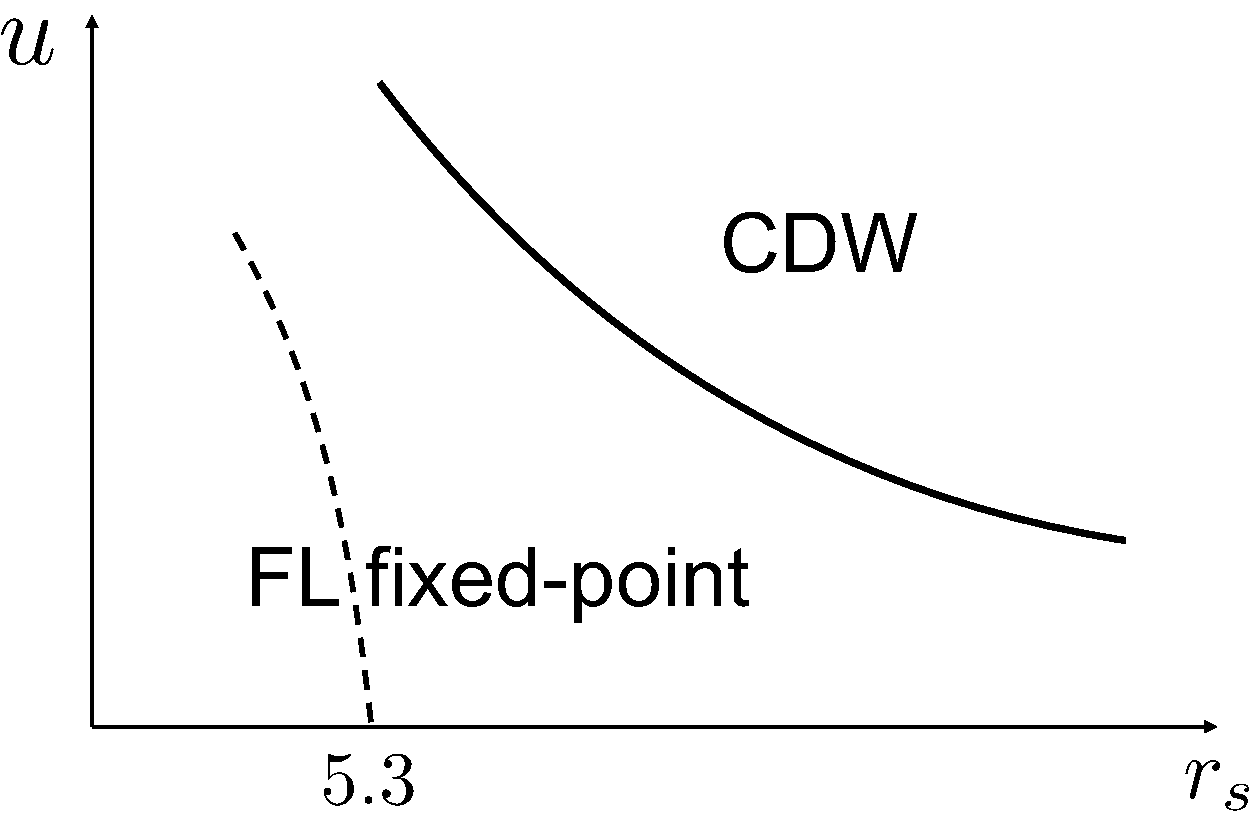
\includegraphics[width=0.9\linewidth]{phase diagram.pdf}
    \caption{Schematic phase diagram of a three-dimensional electron gas with a local attractive interaction. Here $r_s$ is the mean-distance between two electrons that measures the relative strength of the Coulomb repulsion, $u$ is the strength of the local attraction. The quasiparticle interaction (from the vertex correction) together with the local attraction may drive the electron gas to an (incommensurate) charge density wave (CDW). The dash line is where the charge-charge response functions develop universal behaviors below the momentum scale $k_F$.}
    \label{fig:phasediagram}
\end{figure}

As the interaction increases, the structure factor in Eq.\eqref{eq:chi} may develop two types of non-trivial behaviors,
\begin{enumerate}
    \item When $f_0^+=1/\Pi_0^* (0, i\omega_0)$, the dynamic structure factor develops a universal behavior in the limit $\omega_n/v_F \ll v_F q \ll k_F$,
          \begin{equation}
              \chi(q, i\omega_n) \rightarrow \frac{q^2}{4\pi e^2},
          \end{equation}
          which is independent of the Fermi liquid parameters and the local interactions. For generic $f_0^+$, there is a similar universal behavior, but only for the momentum $q<q_{TF}=\sqrt{4\pi e^2 N_F}$, where is the Thomas-Fermi screening wavelength with a renormalized mass $m^*$.

          Similar universal behaviors emerge for other charge-charge response functions as well. For example, dielectric function $\epsilon(q,i\omega_n)=1/(1-f_0^+ \Pi^*_0 (q,i\omega_n))$ diverges in the same limit $\omega_n/v_F \ll v_F q \ll k_F$, diverges. Later, we will show such physics are caused by the emergence of a stable fixed point in the effective field theory of the charge fluctuations.

    \item When $f_0^+ \ll 1/\Pi_0^* (0, i\omega_0)$, there may be a CDW instability at a finite momentum,
          \begin{equation}
              q_c^2=q_{TF}^2\frac{\tilde{\Pi}_0({q_c})}{1-F_0^+ \tilde{\Pi}_0({q_c})},
          \end{equation}
          where $\tilde{\Pi}_0({q_c})=\Pi_0(q_c, i\omega_0)$ is the static polarization at the momentum $q_c$. Note that both the nominator and the denominator in the above equation are negative, ensuring the existence of the critical $q_c$. In general, $q_c$ is not locked to $k_F$ or $2k_F$, indicating the CDW is incommensurate.

          We will be focusing on the soft CDW in the limit $q_c \approx q_{TF}\cdot(-F_0^+)^{-1/2} \ll k_F$. The separation of length scale makes sure that the soft CDW here is a collective mode of low-energy quasiparticles near Fermi surface.

\end{enumerate}

Now we are ready to propose a schematic phase diagram for the electron gas in Fig. \ref{fig:phasediagram}. It is derived from the nontrivial behavior of the structure factor Eq.\eqref{eq:chi} with the estimation of the Landau parameter Eq.\eqref{eq:f}. To summarize, the system undergoes a charged Fermi liquid to CDW quantum phase transition as the interaction increases. The nature of the CDW and the phase transition is not known at this stage. Within the Fermi liquid phase, the charge-charge response functions develops universal behaviors along a line of fixed points.


\appendix
\section{Charged Fermi Liquid Theory}
\label{appendix:FL}

Here we review Landau theory of the charged Fermi liquid.

\subsection{Hedin Equations}

The electron-electron effective interaction is captured by the one-particle-irreducible vertex function $\Gamma_4(k_1, k_2; q)$ where $k_1=(\bk_1, \omega_1)$ and $k_2=(\bk_2, \omega_2)$ are the incoming momenta/frequencies of the two scattered electrons, and $q=(\bq, \Omega)$ is the transfer momentum/frequency between two electrons. For simplicity, we omit the spin index.

We first analysis the analytic structure of the vertex function $\Gamma_4$ in the metallic phase. We expect three different pieces
\begin{equation}
    \Gamma_4=\Gamma_W+\Gamma_{ph}+\Gamma_{irr}
\end{equation}

\begin{itemize}
    \item The first piece is the one-interaction-reducible diagrams $\Gamma_W (k1, k2; q)=\Gamma_3(k_1, q) \cdot W_q \cdot \Gamma_3(k_2, q)$, where $W$ is the renormalized bosonic propagator and $\Gamma_3$ is the one-interaction-irreducible $3$-vertex. It diverges as $4\pi e^2/q^2$ in the limit $q\rightarrow 0, q/\Omega \rightarrow 0$.
    \item The second piece $\Gamma_{ph}(k_1, k_2; q)$ consists of the diagrams which are one-interaction irreducible but particle-hole reducible. In these diagrams, there is at least one pair of electron propagators looks like $G_k G_{k+q}$. Integrating out the internal momentum/frequency $k$, these pairs take different limits as $\bq\rightarrow 0$ and $\Omega \rightarrow 0$. As a result, $\Gamma_{ph}(k_1, k_2; q)$ is finite but non-analytic in the limits $\bq, \Omega \rightarrow 0$.

    \item The third piece $\Gamma_{irr}(k_1, k_2; q)$ are the one-interaction and particle-hole irreducible diagrams. It is analytic in the limits $\bq, \Omega \rightarrow 0$.

    \item It is sometimes convenient to further divide $\Gamma_{irr}$ into three parts $\Gamma_{irr}=\Gamma_W^{ex}+\Gamma_{ph}^{ex}+\delta \Gamma_{irr}$, where the first two terms are the exchange counterparts of $\Gamma_W$ and $\Gamma_{ph}$.
\end{itemize}



The renormalized electron propagator $G$, dressed interaction $W$ and the one-interaction-irreducible $3$-vertex function $\Gamma_3$ can be calculated with the Hedin equations for , respectively,
\begin{align}
    G_k            & =(g^{-1}_k-\Sigma_k)^{-1},                                           \\
    W_q            & =(v_q^{-1}-\Pi_q)^{-1},                                              \\
    \Sigma_k       & =-\sum_q G_k W_q \Gamma_3(k, q),                                     \\
    \label{eq:polar}
    \Pi_q          & =\sum_q G_k G_{k+q} \Gamma_3(k, q),                                  \\
    \Gamma_3(k, q) & =1+\sum_{k'} (\Gamma_{ph}+\Gamma_{irr})_{kk'q}\cdot G_{k'} G_{k'+q}.
\end{align}

We analysis the analytic structure of the above correlation/vertex functions.

\subsection{Green's function}

Near the Fermi surface, the electron propagator can be well approximated with a renormalized free propagator. Therefore, to study low energy physics, it makes sense to write the propagator as,
\begin{equation}
    G_{\bk, i\omega_n}=\frac{Z}{i\omega_n-v_F (k-k_F)}+\text{correction.}.
\end{equation}
or in the imaginary-time representation with $\tau \in [0, \beta)$,
\begin{equation}
    G_{\bk, \tau}=Z(1-n_k)e^{-v_F (k-k_F)\tau}+\text{correction.}.
\end{equation}
where $v_F$ is the physical Fermi velocity, and $k_F$ is the physical Fermi momentum.

\begin{figure}
    \centering
    \label{fig:bubble}
    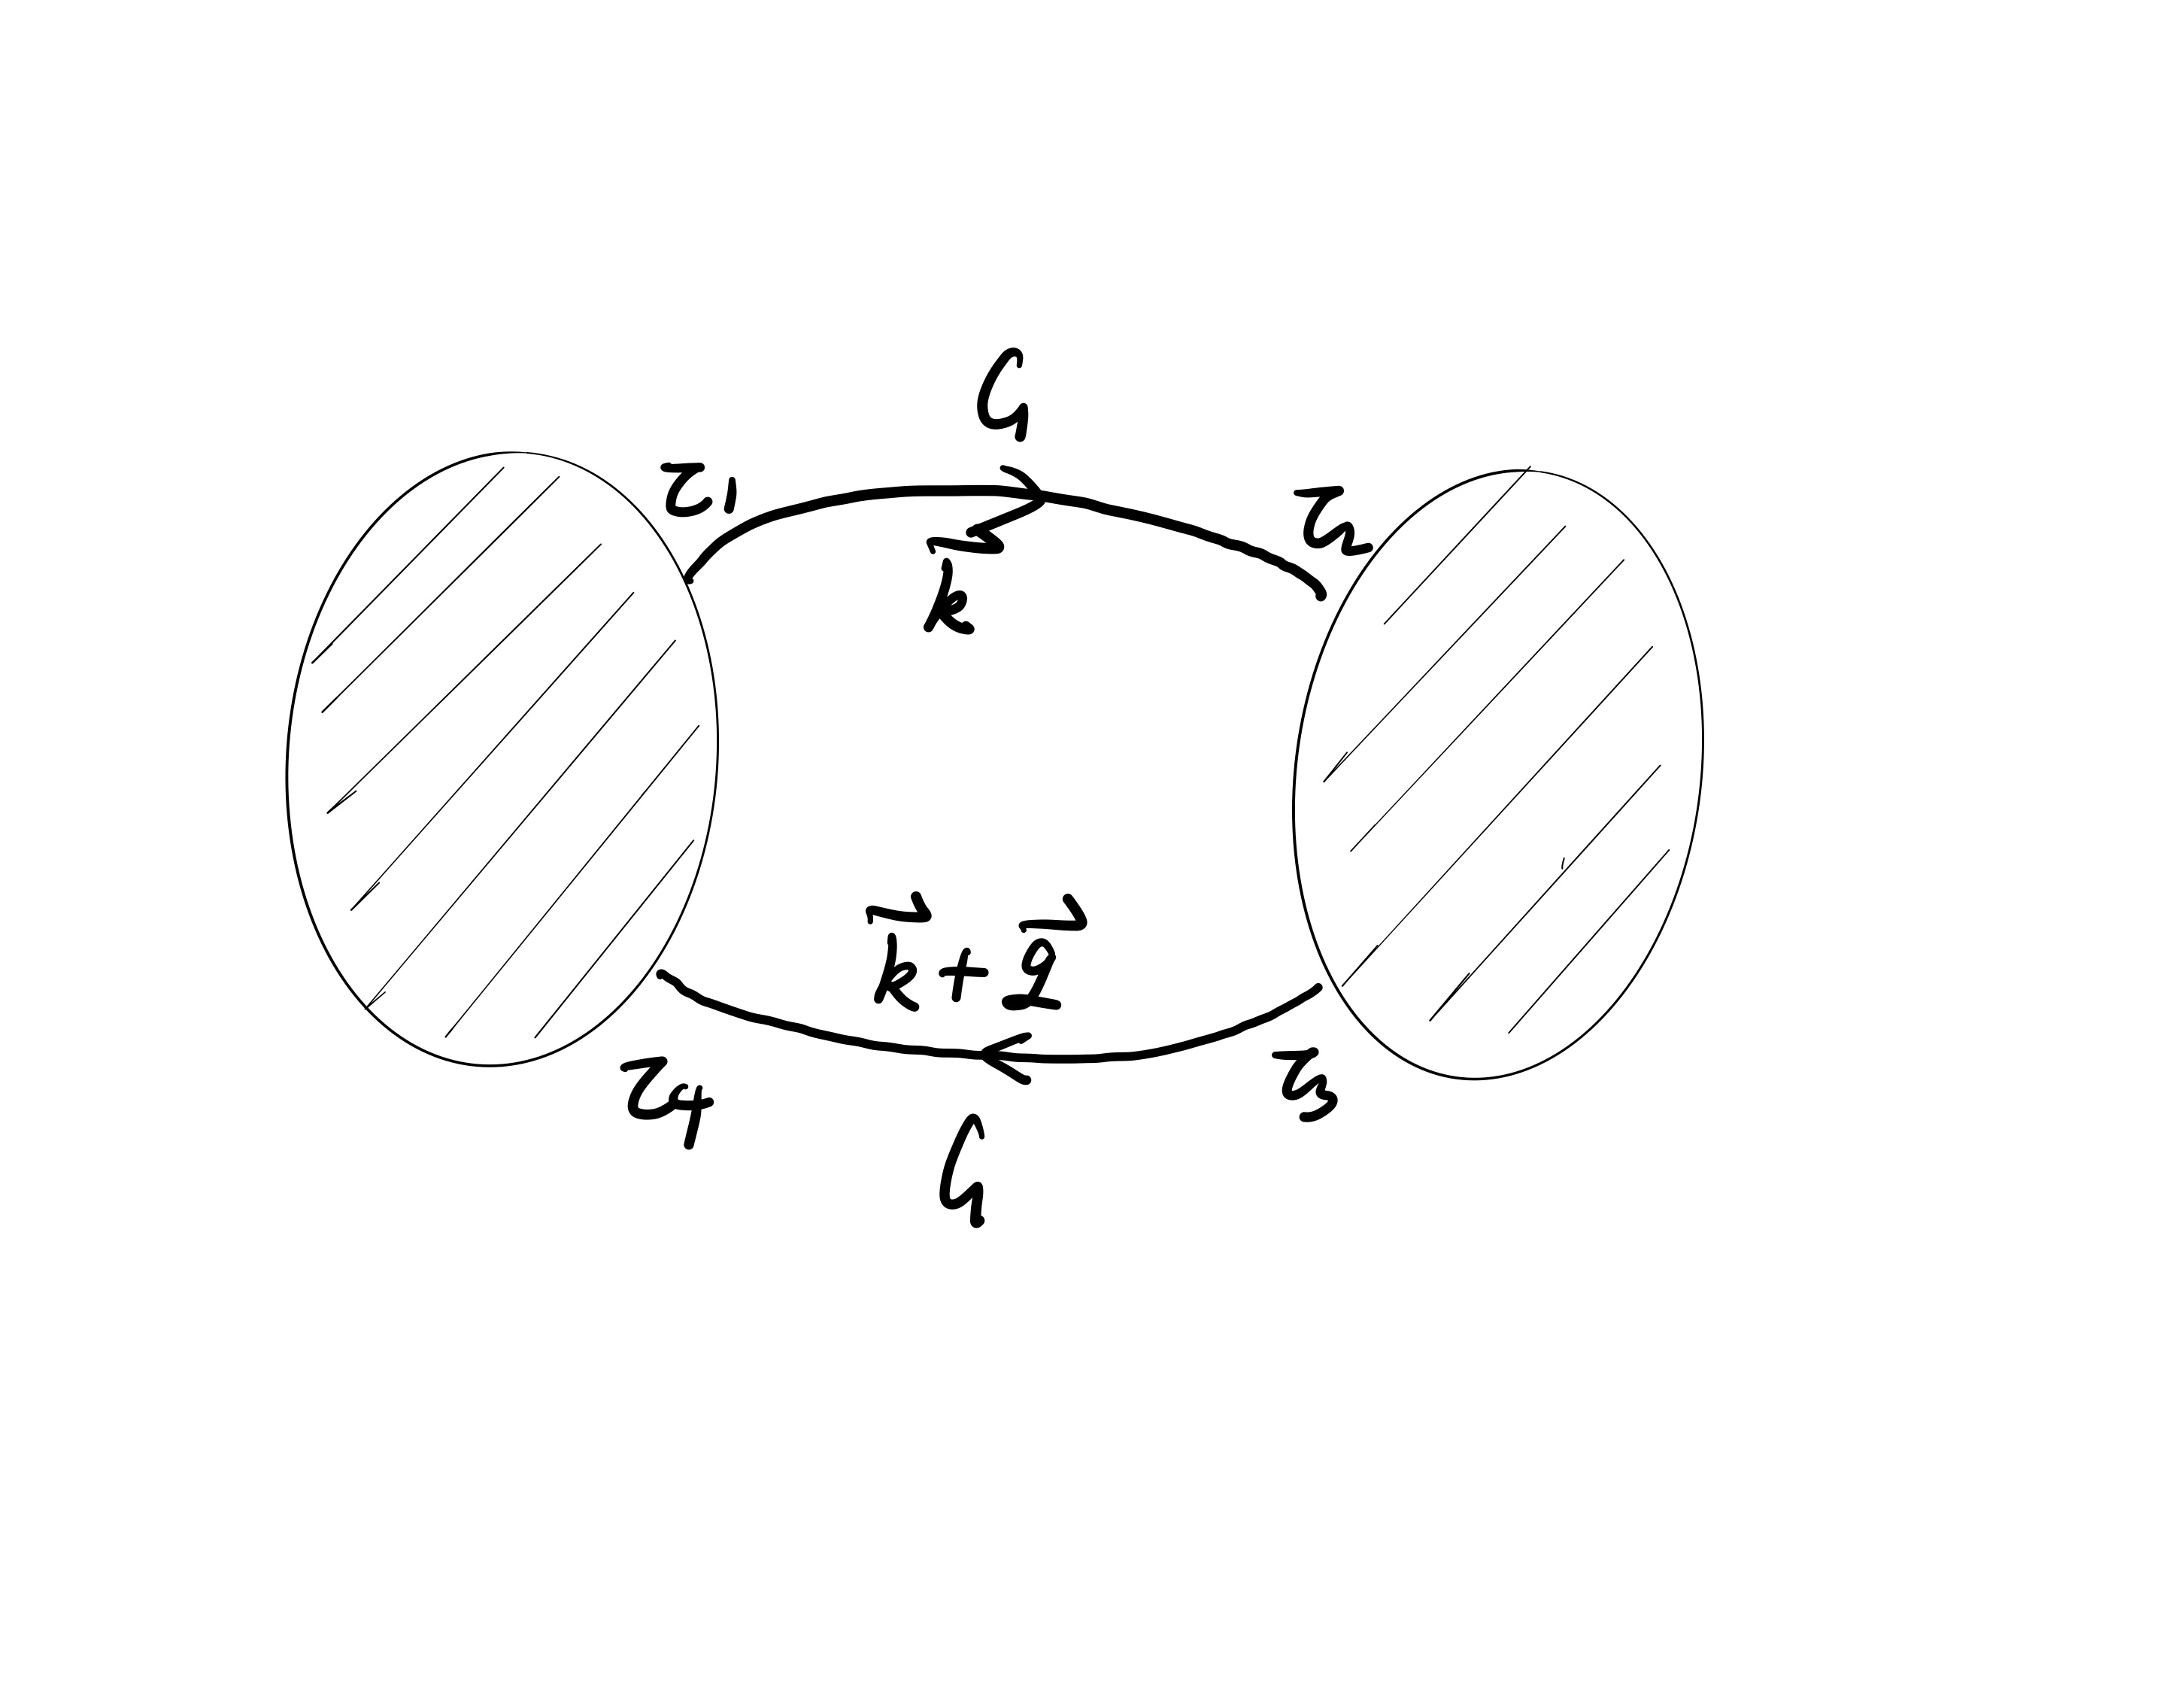
\includegraphics[width=0.7\linewidth]{figure/bubble.jpg}
    \vspace{-1.5cm}
    \caption{Particle-hole pair.}
\end{figure}

The singular part of the propagator leads to a non-analytic contribution in the particle-hole pair (see Fig.\ref{fig:bubble}),
\begin{align}
     & G_{\bk, \tau_2-\tau_1} G_{\bk+\bq,\tau_4'-\tau_3'}=\nonumber                                                                                    \\
     & -Z^2 n_{\bk}(1-n_{\bk+\bq})\cdot e^{-(\epsilon_{\bk+\bq}-\epsilon_{\bk})(\tau_2-\tau_1)} \delta_{\tau_1-\tau_4}\delta_{\tau_2-\tau_3} \nonumber \\
     & +\text{correction}.
\end{align}

At low temperature and with small transfer momentum/frequency $(\bq, i\Omega)$, the internal momentum $\bk$ will be confined near the Fermi surface and the first term will be simplified as,
\begin{equation}
    (GG)_{\bq,i\Omega}=K_{\bq,i\Omega}+\text{correction},
\end{equation}
where the kernel,
\begin{equation}
    K_{\hat{\bk}; \bq,i\Omega}=\frac{Z^2\hat{\bk}\cdot \bq}{i\Omega-v_F \hat{\bk}\cdot \bq}.
\end{equation}

%where we represent the object in the imaginary-time instead of the Matsubara frequency for clarity. The first term, namely the polarization of free electrons, is non-analytic in the limit $\bq, \Omega \rightarrow 0$,
%\begin{equation}
%\label{eq:free_polar}
%\Pi_{\bq, i\omega}^{free}=\left\{
%                \begin{array}{ll}
%                0, \;\;\;\;\;\;\;\;\;\;\; \bq=0, i\omega \rightarrow 0 \\
%                  \frac{mk_F}{2\pi^2}\cdot S, \;\; \bq\rightarrow 0, i\omega=0
%                \end{array}
%              \right.
%\end{equation}

\subsection{Forward-Scattering Electron-Electron Interaction $\Gamma_4$}
\label{appendix:renormalization}

We now give the analytic structure of the electron-electron interaction near the Fermi surface. We first define the $4$-vertex in the limit $\bq, \Omega\rightarrow 0$ and $\bq/\Omega \rightarrow 0$ as,
\begin{equation}
    \label{eq:gamma_4_omega}
    \Gamma_4^\Omega (k_1, k_2; \bq)=\frac{1}{Z^2}v_q+\Gamma_{p+i}^\Omega(k_1, k_2),
\end{equation}
where $\Gamma_{p+i}$ is an abbreviation of $\Gamma_{ph}+\Gamma_{irr}$. The first term is from the one-interaction-reducible term $\Gamma_W (k1, k2; q)=\Gamma_3(k_1, q) \cdot W_q \cdot \Gamma_3(k_2, q)$. Due to the charge conservation\cite{agd}, in this limit, $W_q=v_q$ and $\Gamma_3(k_1, q)=1/Z$.

The forward-scattering full vertex function is given by,
\begin{align}
    \Gamma_4 & (k_1, k_2; \bq, i\Omega)=\Gamma_4^\Omega(k_1, k_2; \bq) \nonumber \\&
    +\frac{Z^2k_F^2}{(2\pi)^D} \int_{\Omega_k} \Gamma_4^\Omega(k_1, k; \bq)\frac{\hat{\bk}\cdot \bq}{i\Omega-v_F \hat{\bk}\cdot \bq}\Gamma_4(k, k_2; \bq, i\Omega).
\end{align}
where the momentum/frequency $k=(\bk_F, i\omega_0)$ is on the Fermi surface.

If we only consider the one-interaction-irreducible components,
\begin{align}
    \Gamma & _{p+i}(k_1, k_2; \bq, i\Omega)=\Gamma_{p+i}^\Omega(k_1, k_2) \nonumber                                                                                             \\
           & +\frac{Z^2k_F^2}{(2\pi)^D} \int_{\Omega_k} \Gamma_{p+i}^\Omega(k_1, k)\frac{\hat{\bk}\cdot \bq}{i\Omega-v_F \hat{\bk}\cdot \bq}\Gamma_{p+i}(k, k_2; \bq, i\Omega).
\end{align}

In the limit $\bq, \Omega\rightarrow 0$ and $\Omega/\bq \rightarrow 0$, the $4$-vertex function corresponds to the forward scattering amplitude. Again, it consists of one-interaction-reducible part and the irreducible part.

The one-interaction-reducible contribution $\Gamma^3_{\bq, i\Omega} W_{\bq, i\Omega} \Gamma^3_{\bq, i\Omega}$, where the $3$-vertex $\Gamma_3^{\bq, i\Omega}$ is given in Eq.\eqref{eq:gamma3} and the dressed interaction $W_{\bq, i\Omega}$ is given in Eq. \ref{eq:interaction}. Note that this term is a function of the transfer momentum/frequency only.

The one-interaction-irreducible part is,
\begin{equation}
    \label{eq:gamma4pi}
    \Gamma_{p+i}^q(k_1, k_2)=\Gamma_{p+i}^\Omega-\frac{Z^2m^* k_F}{(2\pi)^D} \int_{\Omega_k} \Gamma_{p+i}^\Omega(k_1, k)\Gamma_{p+i}^q(k, k_2),
\end{equation}
where $m^*$ is the effective mass of the quasiparticle.

For fermions carrying $S=1/2$,
\begin{equation}
    \Gamma_{p+i}=\Gamma_{p+i}^{+}+\Gamma_{p+i}^{-}\sigma_1\cdot\sigma_2,
\end{equation}
where the first term is spin symmetric, while the second term is antisymmetric. Then Eq.\eqref{eq:gamma4pi} decouples into,
\begin{equation}
    \label{eq:gamma4pi_spin}
    \Gamma_{p+i}^{q,\pm}(k_1, k_2)=\Gamma_{p+i}^{\Omega,\pm}-\frac{2 Z^2m^* k_F}{(2\pi)^D} \int_{\Omega_k} \Gamma_{p+i}^{\Omega,\pm}(k_1, k)\Gamma_{p+i}^{q,\pm}(k, k_2),
\end{equation}

If both $k_1, k_2$ are on the Fermi surface, $\Gamma_4^\Omega (k_1, k_2)$ corresponds to the Landau quasiparticle interaction (for the effective Hamiltonian formulation),
\begin{equation}
    \label{eq:F}
    \frac{Z^2 m^* k_F}{\pi^2}\Gamma_{p+i}^\Omega (k_1, k_2)=\sum_l (2l+1)(F_l^++F_l^-\sigma_1\cdot\sigma_2) P_l(\cos\theta_{12}),
\end{equation}
while $\Gamma_4^q (k_1, k_2)$ corresponds to the scattering amplitude,
\begin{equation}
    \frac{Z^2 m^* k_F}{\pi^2}\Gamma_{p+i}^q (k_1, k_2)=\sum_l (2l+1)(A_l^++A_l^-\sigma_1\cdot\sigma_2) P_l(\cos\theta_{12}).
\end{equation}

In three-dimensions $D=3$, use the addition formula,
\begin{equation}
    P_l(\cos\theta_{12})=\frac{4\pi}{2l+1} \sum_{m=-l}^{l} Y_{lm}(\hat{k}_1) Y^*_{lm}(\hat{k}_2),
\end{equation}
where the spherical harmonics normalizes to one,
\begin{equation}
    \int_{\Omega_{\hat{k}}}  Y_{lm}(\hat{k}) Y^*_{l'm'}(\hat{k})=\delta_{l,l'}\delta_{m, m'}.
\end{equation}
Eq.\eqref{eq:gamma4pi_spin} simplifies to,
\begin{equation}
    A_l^\pm=F_l^\pm-F_l^{\pm}A_l^\pm,
\end{equation}
which has a simple solution,
\begin{equation}
    A_l^\pm=\frac{F_l^\pm}{1+F_l^\pm}
\end{equation}

\subsection{Dressed Interaction $W$}

The physical polarization has a similar non-analytic structure in the limit $\bq, i\Omega \rightarrow 0$,
\begin{equation}
    \label{eq:polar}
    \Pi_{\bq, i\omega}=\Gamma_3^{\Omega}K_{\bq, i\omega} \Gamma_3^q(\bq, i\omega)=\frac{1}{Z^2}K_{\hat{\bk}; \bq, i\omega}\cdot(1-\Gamma_{p+i}^\Omega \cdot K_{\bq, i\omega})^{-1}_{\hat{\bk}}
\end{equation}
where the $3$-vertex $\Gamma_3^{\Omega, q}$ is given in Eq.\eqref{eq:gamma3}, and the $4$-vertex $\Gamma^{\Omega}_{ph+irr}$ is the one-interaction-irreducible quasiparticle interaction, which is given by Eq.\ref{eq:gamma_4_omega}. There are two interesting limits,
\begin{equation}
    \Pi_{\bq, i\omega}=\left\{
    \begin{array}{ll}
        0, \;\;\;\;\;\;\;\; \bq=0, i\omega \rightarrow 0 \\
        -n^2\kappa, \;\; \bq\rightarrow 0, i\omega=0
    \end{array}
    \right.
\end{equation}
where $n$ is the electron density and $\kappa$ is the proper charge compressibility.

Use Eq.\eqref{eq:F}, the proper compressibility has a simple expression,
\begin{equation}
    \frac{\kappa}{\kappa_0}=\frac{m^*}{m}\frac{1}{1-\Gamma_{p+i}^\Omega \cdot K_{\bq, i\omega}}=\frac{m^*}{m}\frac{1}{1+F_0^+}
\end{equation}

The dressed interaction, or the renormalized bosonic propagator, is given by,
\begin{equation}
    \label{eq:interaction}
    W_{\bq, i\omega}=\left\{
    \begin{array}{ll}
        v_q, \;\;\;\;\;\;\;\;\;\;\;\;\;\;\;\;\;\; \bq=0, i\omega \rightarrow 0 \\
        v_q/(1+v_q n^2 \kappa), \;\; \bq\rightarrow 0, i\omega=0
    \end{array}
    \right.
\end{equation}
where $\kappa$ is referred as the proper compressibility of the electron gas.

\subsection{$3$-Vertex $\Gamma_3$}

The behavior of the $3$-vertex in the limit $\bq, \Omega \rightarrow 0$ is fixed by the Ward identity associated with the charge conservation (Note that some approximation may violate it)
\begin{align}
    \label{eq:gamma3}
    \Gamma_3 & (\bk, i\omega; \bq, i\Omega)= \nonumber \\
             & \left\{
    \begin{array}{ll}
        \Gamma_3^\Omega= \frac{\partial G^{-1}}{\partial i\omega_n}=\frac{1}{Z}, \;\;\;\;\;\;\;\;\;\;\;\;\; \bq = 0, i\Omega \rightarrow 0 \\
        \Gamma_3^q =(1-\Gamma_{p+i}^\Omega \cdot K_{\bq, i\omega})^{-1}\cdot\Gamma_3^\Omega,
        \bq \rightarrow 0, i\Omega =0
    \end{array}
    \right.
\end{align}

With Landau parameter, $\Gamma_3^q$ has a simple expression,
\begin{equation}
    \Gamma_3^q=\frac{1}{Z}\frac{1}{1+F_0^+}.
\end{equation}
One may refer to Ref. \citenum{agd} for a detailed derivation. The $3$-vertex has a remarkable feature in the forward scattering channel: it is independent of the incoming momentum/frequency of the electron (not only the amplitude, but also the angle).


\section{Microscopic Theory of the Kukkonen-Overhauser Interaction}

The Kukkonen-Overhauser ansatz is a phenomenological theory for the effective electron-electron interaction in a Coulomb gas\cite{kukkonen}. In Ref.\citenum{vignale1}, the authors attempt to construct a microscopic theory for the Kukkonen-Overhauser ansatz.  However, this theory resorts to a uncontrolled approximation in which the authors assume that the particle-hole-irreducible vertex function depends only on the momentum transfer along the particle-hole channel ("local" approximation). The operation definition of such approximation is not absent. As a result, it is impossible to calculate the high order corrections within the current form of the theory. To fix this problem, we will propose a microscopic theory for the KO interaction without relying on uncontrolled approximation. Our theory can be regarded as a generalization of the Landau Fermi liquid theory to non-forward scattering process.

Following the reasoning of the Fermi liquid theory, we split the 1PI $4$-point vertex function $\Gamma^4$ into a particle-hole-irreducible vertex function $\Gamma^{ph}$ and the remaining reducible part,
\begin{equation}
    \Gamma^4_{12;34}=\Gamma^{ph}_{1,2;3,4}+\int_{1',2',3',4'}\Gamma^{ph}_{1,1';3,3'}G_{3',2'}G_{4',1'}\Gamma^4_{2',2;4',4},
\end{equation}
where the label include momentum, frequency and the spin index. $G_{55'}$ are the fully dressed electron propagator from $5$ to $5'$.

The particle-hole pair can be split into a non-analytic term and a regular correction,
\begin{equation}
    G_{3',2'}G_{4',1'}=z^2\Pi^*_{0; 1',2'}\delta_{1',3'}\delta_{2',4'}+\phi_{3',4';1',2'},
\end{equation}

One can prove that,
\begin{equation}
    \Gamma^4_{12;34}=F_{1,2;3,4}+\int_{1',2',3',4'}F_{1,1';3,1'}z^2\Pi^*_{1',2'}\Gamma^4_{2',2;2',4},
\end{equation}
where,
\begin{equation}
    F_{1,2;3,4} = \Gamma_{ph}+\Gamma_{ph}\phi\Gamma_{ph}+\Gamma_{ph}\phi\Gamma_{ph}\phi\Gamma_{ph}+...
\end{equation}



\section{Problem of Double Counting}

By definition, the renormalized field theory at the tree level should exactly reproduces the quasiparticle scattering amplitude, which is given by the $1PI$ $4$-point vertex function averaged on the Fermi surface,
%\begin{equation}
%    z^2 \left[\Gamma_4(k_1, k_2, q\rightarrow 0)\right]_{k_F, l=0}^+ = \frac{v_q+f^+}{1-(v_q+f^+) \Pi_0^*}\delta_{\alpha\beta}\delta_{\gamma\delta}, 
%\end{equation}
\begin{align*}
      & z^2 \left[\Gamma_4(k_1, k_2, q\rightarrow 0)\right]_{k_F, l=0}                                                                                                     \\
    = & \frac{v_q+f^+}{1-(v_q+f^+) \Pi_0^*}\delta_{\alpha\beta}\delta_{\gamma\delta}+\frac{f^-}{1-f^- \Pi_0^*}\vec{\sigma}_{\alpha\beta}\cdot \vec{\sigma}_{\gamma\delta},
\end{align*}
where $q=(\bq, i\Omega)$ should be small compared to the Fermi momentum and Fermi energy. The spin indices $\alpha, \gamma$ are for the two incoming electrons, while $\beta, \delta$ are for the outing ones.

The field theory has three tree level contributions to the scattering amplitude:
\begin{enumerate}
    \item Two quasiparticle exchanges an intermediate boson, which generates a contribution,
          \begin{equation}
              W(q) = \frac{v_q+f^+}{1-(v_q+f^+) \Pi_0^*}\delta_{\alpha\beta}\delta_{\gamma\delta}+\frac{f^-}{1-f^- \Pi_0^*}\vec{\sigma}_{\alpha\beta}\cdot \vec{\sigma}_{\gamma\delta},
          \end{equation}
          %    \begin{equation}
          %        W(q\rightarrow 0)=\frac{4\pi e^2}{(1-f^+\Pi_0^*)q^2-4\pi e^2 \Pi_0^*}\delta_{\alpha\beta}\delta_{\gamma\delta}.
          %    \end{equation}
          Note that this contribution coincides with the quasiparticle scattering amplitude in the long-wave-length limit, meaning all other scattering amplitude contributions from the theory must be exactly cancel in this limit.

    \item Two quasiparticle exchanges an intermediate boson, then permutates with each other. It generates a contribution,

          \begin{equation}
              \left[W_{ex}\right]_{k_F, l=0}=-\bar{w}^+\delta_{\alpha\delta}\delta_{\gamma\beta}-\bar{w}^-\vec{\sigma}_{\alpha\delta}\cdot \vec{\sigma}_{\gamma\beta}
          \end{equation}
          where,
          \begin{equation}
              w^+(\theta_{12})=\frac{v_q+f^+}{1-(v_q+f^+) \Pi_0^*}|_{q=2k_F\text{sin}^2(\frac{\theta_{12}}{2})},
          \end{equation}
          and,
          \begin{equation}
              w^-(\theta_{12})=\frac{f^-}{1-f^- \Pi_0^*}|_{q=2k_F\text{sin}^2(\frac{\theta_{12}}{2})},
          \end{equation}
          and we define $\bar{w}^{\pm}$ as the average of $w^{\pm}(\theta_{12})$ on the Fermi surface,
          \begin{equation}
              \bar{w}^{\pm}=\int w^{\pm}(\theta_{12})d\Omega .
          \end{equation}

          %\begin{equation}
          %    W_{ex}(q\rightarrow 0)=-\int d\Omega \frac{4\pi e^2}{(1-f^+\Pi_0^*)k_F^2\text{sin}^2\frac{\theta}{2}-4\pi e^2 \Pi_0^*}\delta_{\alpha\delta}\delta_{\gamma\beta} 
          %\end{equation}
          Note that the the spin indices $\beta \leftrightarrow \delta$ have been exchanged. To match with the spin indices of the external legs, one needs to reparameterize it,
          \begin{equation}
              \delta_{\alpha\delta}\delta_{\gamma\beta}=\frac{1}{2}\delta_{\alpha\beta}\delta_{\gamma\delta}+\frac{1}{2}\vec{\sigma}_{\alpha\beta}\cdot \vec{\sigma}_{\gamma\delta},
          \end{equation}
          where we use the identity $\vec{\sigma}_{\alpha\beta}\cdot \vec{\sigma}_{\gamma\delta}=2 \delta_{\alpha \delta} \delta_{\beta \gamma}-\delta_{\alpha \beta} \delta_{\gamma \delta}$. Similarly,
          \begin{equation}
              \vec{\sigma}_{\alpha\delta}\cdot \vec{\sigma}_{\gamma\beta}=\frac{3}{2}\delta_{\alpha\beta}\delta_{\gamma\delta}-\frac{1}{2}\vec{\sigma}_{\alpha\beta}\cdot \vec{\sigma}_{\gamma\delta}
          \end{equation}

          We conclude the contribution to the scattering amplitude,
          \begin{equation}
              \label{eq:exchange_kF}
              \left[W_{ex}\right]_{k_F, l=0}=-\frac{\bar{w}^+ +3\bar{w}^-}{2}\delta_{\alpha\beta}\delta_{\gamma\delta}-\frac{\bar{w}^+-\bar{w}^-}{2}\vec{\sigma}_{\alpha\beta}\cdot \vec{\sigma}_{\gamma\delta}
          \end{equation}
          %\begin{equation}
          %    W_{ex}^+(q\rightarrow 0)=-\frac{1}{2}\int d\Omega \frac{4\pi e^2}{(1-f^+\Pi_0^*)k_F^2\text{sin}^2\frac{\theta}{2}-4\pi e^2 \Pi_0^*}\delta_{\alpha\beta}\delta_{\gamma\delta} 
          %\end{equation}

    \item Two quasiparticles has a contact interaction, assume it takes a form,
          \begin{equation}
              u(\theta_{12})=u^+(\theta_{12})\delta_{\alpha\beta}\delta_{\gamma\delta}+u^-(\theta_{12})\vec{\sigma}_{\alpha\beta}\cdot \vec{\sigma}_{\gamma\delta}
          \end{equation}

          If we assume that $u^{\pm}(\theta_{12})$ is a constant, then the sum of direct and exchange contribution is
          \begin{equation}
              U_{\alpha\beta\gamma\delta}=\frac{u^+-3u^-}{2}\delta_{\alpha\beta}\delta_{\gamma\delta}-\frac{u^+-3u^-}{2}\vec{\sigma}_{\alpha\beta}\cdot \vec{\sigma}_{\gamma\delta},
          \end{equation}
          which only has one free parameter $u^+-3u^-$. We may fix this parameter by requiring the contact term completely cancel the spin-symmetric part of the exchange contribution in Eq.\eqref{eq:exchange_kF}, namely
          \begin{equation}
              u^+-3u^-=\bar{w}^+ +3\bar{w}^-.
          \end{equation}
          This choice will leads to a net spin-asymmetric contribution,
          \begin{equation}
              (\bar{w}^++\bar{w}^-)\vec{\sigma}_{\alpha\beta}\cdot \vec{\sigma}_{\gamma\delta}.
          \end{equation}
          Such correction makes the scattering amplitude and the Landau parameter unbalanced at the tree level. If we require it to vanish, we then have an additional constraint which fixes $f^-$,
          \begin{equation}
              \bar{w}^{-} = -\bar{w}^{+}
          \end{equation}

          By fixing the spin-symmetric scattering amplitude to be physical, we are forced to introduce $f^-$ and $u$ together to make the theory self-consistent.

\end{enumerate}

\bibliographystyle{apsrev4-1}
\bibliography{ref}

\end{document}